\documentclass[12pt,superscriptaddress,preprint,nofootinbib,aps,prd]{revtex4-2}

% Core packages
\usepackage[utf8]{inputenc}
\usepackage{amsmath,amssymb,mathtools}
\usepackage{amsthm}
\usepackage{graphicx}
\usepackage{xcolor}
\usepackage{url}
\usepackage{enumerate}
\usepackage{cancel}
\usepackage{tikz}
\usetikzlibrary{positioning,arrows.meta}
\usepackage{tikz-cd}
\usepackage[title]{appendix}
\usepackage{siunitx}
\sisetup{per-mode=symbol}
\usepackage{mathrsfs}
\usepackage{import}
\usepackage{enumitem}
\usepackage{booktabs}

% ----------------------------------------------------------------------------
% Submission-oriented edits (no red/blue issue text in compiled output)
% ----------------------------------------------------------------------------

% Units
\DeclareSIUnit\au{a.u.}
\DeclareSIUnit\angstrom{\text{\AA}}

% Ensure compatibility with apsrev4-2 .bbl helper macros
\makeatletter
\let\href@noop\relax
% Fix TOC spacing for Roman numerals (guarded for revtex4-2 compatibility)
\@ifundefined{l@section}{}{%
  \renewcommand*\l@section{\@dottedtocline{1}{0em}{3em}}%
  \renewcommand*\l@subsection{\@dottedtocline{2}{1.5em}{4em}}%
  \renewcommand*\l@subsubsection{\@dottedtocline{3}{3.5em}{5em}}%
}
\makeatother

% Theorem environments
\newtheorem{theorem}{Theorem}[section]
\newtheorem{lemma}[theorem]{Lemma}
\newtheorem{axiom}[theorem]{Axiom}
\newtheorem{proposition}[theorem]{Proposition}
\newtheorem{corollary}[theorem]{Corollary}
\newtheorem{definition}[theorem]{Definition}
\newtheorem{remark}[theorem]{Remark}
\newtheorem{observation}[theorem]{Observation}
\newtheorem{conjecture}[theorem]{Conjecture}
\renewcommand{\qedsymbol}{$\square$}

% Macros
\newcommand{\Rec}{\mathrm{Recognition}}
\newcommand{\N}{\mathbb{N}}
\newcommand{\NN}{\N} % alias; avoid duplicate definitions
\newcommand{\id}{\mathrm{id}}
\newcommand{\Id}{\id} % alias; avoid duplicate definitions
\newcommand{\Post}{\mathsf{Post}}
\newcommand{\RR}{\mathbb{R}}
\newcommand{\ZZ}{\mathbb{Z}}
\newcommand{\Ccoh}{\mathcal{C}} % coherence threshold (calligraphic C; kernel amplitude uses italic C)

% Footnote style
\renewcommand{\thefootnote}{\fnsymbol{footnote}}

% Section and subsection numbering format (I, II, III for sections; II.1, II.2, etc. for subsections)
\makeatletter
% Save class defaults so \appendix can label appendices (A, B, ...) correctly.
\let\RC@origthesection\thesection
\let\RC@origthesubsection\thesubsection
\makeatother
\renewcommand{\thesection}{\Roman{section}}
\renewcommand{\thesubsection}{\thesection.\arabic{subsection}}
\makeatletter
\renewcommand{\p@subsection}{} % Prevent double section number in \ref (fixes §II II.1 issue)
\makeatother

% Hyperref must remain last (package load)
\usepackage[bookmarks,linktocpage,pdfpagelabels,plainpages=false,
hyperfigures,linkcolor=blue,citecolor=blue]{hyperref}
\hypersetup{colorlinks=true}

\begin{document}

\title[Toward a Discrete Informational Framework for Classical Gravity]{\texorpdfstring{Toward a Discrete Informational Framework for Classical Gravity: \\
Foundations, Constraints, and Testable Predictions}{Toward a Discrete Informational Framework for Classical Gravity: Foundations, Constraints, and Testable Predictions}}

\author{Jonathan Washburn}
\email{washburn@recognitionphysics.org}
\affiliation{Recognition Physics Institute, Austin, Texas, USA}

\author{Megan Simons}
\affiliation{Recognition Physics Institute, Austin, Texas, USA}

\author{Elshad Allahyarov}
\email{elshad.allakhyarov@case.edu}
\affiliation{Recognition Physics Institute, Austin, Texas, USA}
\affiliation{Institut f\"ur Theoretische Physik II: Weiche Materie, Heinrich-Heine Universit\"at D\"usseldorf,
Universit\"atsstrasse 1, 40225 D\"usseldorf, Germany}
\affiliation{Theoretical Department, Joint Institute for High Temperatures, Russian Academy of Sciences (IVTAN),
13/19 Izhorskaya street, Moscow 125412, Russia}
\affiliation{Department of Physics, Case Western Reserve University, Cleveland, Ohio 44106-7202, United States}

\begin{abstract}
We present a discrete informational framework for gravity starting from an informational axiom and confront it with galaxy rotation curves. The framework posits scale-free ledger-closure latency, which induces a fractional-memory mechanism. This mechanism produces scale-dependent gravitational response. Empirically, an effective disk-closure model with three free parameters fits 147 SPARC rotation curves at $\chi^2/\nu = 1.07$, showing competitive performance against MOND and $\Lambda$CDM. Candidate parameter values motivated by self-similarity arguments are discussed, but this manuscript treats parameters as free to keep the empirical interface logically independent of the conjectured forcing chain.
\end{abstract}

\maketitle

\tableofcontents

%=============================================================================
\section{Introduction}
\label{sec:intro}
%=============================================================================

\subsection{Motivation and Context}

Unifying general relativity \cite{einstein1916,MTW1973} with quantum mechanics \cite{dirac1930,dewitt1967} remains a central challenge in theoretical physics. Despite GR's empirical success at classical scales \cite{wald1984,will1993}, a consistent quantum theory of gravity is elusive. This has motivated exploring discrete spacetime structures \cite{wheeler1990,rovelli2004,penrose1971,thooft1993}---loop quantum gravity \cite{rovelli2004,ashtekar2004}, causal sets \cite{bombelli1987,sorkin2003}, Regge calculus \cite{regge1961}, and related programs \cite{konopka2006}. Information-theoretic perspectives \cite{bekenstein1973,hawking1975,thooft1993,susskind1995,maldacena1999,wheeler1990} inspire emergent-gravity proposals \cite{verlinde2011,padmanabhan2010,jacobson1995}, though most lack falsifiable predictions at accessible scales.

Astrophysically, $\Lambda$CDM successfully explains large-scale structure \cite{planck2018,bennett2003} but encounters persistent galactic-scale tensions: core-cusp discrepancies, missing satellites, and too-big-to-fail problems \cite{bullock2017,weinberg2015,moore1999,klypin1999,boylankolchin2011}. MOND \cite{milgrom1983} empirically fits rotation curves \cite{famaey2012,mcgaugh2016,lelli2017} yet lacks fundamental theoretical underpinnings and struggles with cluster-scale observations \cite{clowe2006,sanders2003}. This situation motivates exploring whether galactic dynamics might provide empirical access to discrete quantum-gravity structures.

\subsection{Overview (nontechnical)}

This paper explores a simple idea: if gravitational response is mediated by a discrete ``ledger'' of recognition/closure events, then \emph{delays} in ledger closure can act like a memory of past sources. In the continuum, such memory naturally produces a \emph{scale-dependent} modification to the Newtonian response that is mild (power-law) rather than introducing a new acceleration scale with a sharp transition.

\subsection{Main Results (technical summary)}

This paper presents three key advances:

\paragraph{(1) Framework and kernel derivation.}
We construct a discrete ledger framework starting from an informational axiom and obtain a \emph{candidate} modified-gravity kernel through scale-free ledger-closure latency. The kernel takes the form $w(k)=1+C(k_0/k)^\alpha$ with $X$-only reciprocity ($X:=k c\tau_0/a$), corresponding to a nonlocal Green's function where the modification scales as $\delta\Phi(r)\propto r^{\alpha-1}$ for point sources.

\paragraph{(2) Parameter constraints (conditional).}
We discuss \emph{candidate parameter relations motivated within a constrained informational framework}: self-similarity arguments suggest values near $\alpha \approx 0.191$ and $C \approx 0.382$, with the golden ratio appearing as a fixed point of a two-scale decomposition. We state explicitly which additional assumptions would be required for any such relation to become theorem-level and otherwise treat these steps as conditional/hypothesis-level.

\paragraph{(3) Empirical validation against galaxy rotation curves.}
An effective disk-closure model with three free parameters fits 147 SPARC galaxies at $\chi^2/\nu = 1.07$. Bayesian model comparison shows competitive performance against MOND ($\Delta\ln Z \approx +1.8$) and $\Lambda$CDM ($\Delta\ln Z \approx +2.7$), with best-fit values consistent (within $1\sigma$) with the candidate relations discussed above.


\subsection{Approach and Framework}

We now introduce the ledger framework as a minimal discrete bookkeeping model for recognition events. In this context a ``ledger'' is simply a directed, integer-valued accounting of interactions between localized degrees of freedom; the purpose of this setup is to make conservation and locality explicit before any continuum limits are taken.

The ledger program starts from an informational axiom: a recognition event requires non-empty data, $\neg \exists\, \Rec(\emptyset, \emptyset)$. To obtain a concrete discrete dynamics, we additionally \emph{postulate} structural constraints (A1--A5) capturing non-triviality, locality, integrality, conservation, and minimality. MP motivates (but does not by itself entail) these further assumptions.

Together, these postulates define a discrete bookkeeping system with integer postings on directed edges, atomic ticks, and closed-chain neutrality (a discrete Kirchhoff law). A unique symmetric cost functional is used throughout: $J(x) = \frac{1}{2}(x + x^{-1}) - 1$. Discrete exterior calculus (DEC) provides a bridge to continuum Poisson equations in appropriate limits. Topological synchronization arguments conjecture spatial dimension $D=3$ from gap-pattern constraints.


\subsection{Current Status and Scope}

The paper presents a structured argument chain with identified gaps. Table~\ref{tab:forcing-chain} displays a forcing chain from the Recognition Composition Law (RCL) to the golden-ratio ILG parameters, with explicit status for each step. (We label these as ``FC'' steps to avoid confusion with the appendix theorem numbering.)

\begin{table}[h]
\centering
\small
\setlength{\tabcolsep}{4pt}
\begin{tabular}{>{\raggedright\arraybackslash}p{1.5cm} >{\raggedright\arraybackslash}p{8.5cm} >{\raggedright\arraybackslash}p{2.6cm} >{\raggedright\arraybackslash}p{2.4cm}}
\toprule
\textbf{Step} & \textbf{Claim} & \textbf{Status} & \textbf{Dependency} \\
\midrule
FC0 & RCL $\to$ unique $J(x) = \tfrac{1}{2}(x+x^{-1})-1$ & \textbf{Proved (this paper)} & A1--A3 \\
FC1 & $J(0^+) \to \infty$ (MP derived) & Motivated & FC0 \\
FC2 & Discreteness (continuous unstable under $J$) & Motivated & FC0 \\
FC3 & $J$-symmetry $\to$ double-entry ledger & Motivated & FC0 \\
FC4 & Observables require recognition events & Conjectured & FC0--FC3 \\
FC5 & Self-similarity $\to$ $\varphi = (1{+}\sqrt{5})/2$ & Conditional (Prop.~\ref{prop:phi-from-selfsimilarity}) & FC2--FC4 \\
FC6 & $2^D$ coverage $\to$ 8-tick period ($D{=}3$) & Motivated & FC5 \\
FC7 & Gap-45 sync $\to$ dimension $D{=}3$ unique & Motivated & FC6 \\
\midrule
A6 & Scale-free latency $\to$ fractional memory & \textbf{Assumption} & --- \\
A7 & Causal closure $\to$ $\omega \sim k$ & \textbf{Assumption} & --- \\
\midrule
ILG-$\alpha$ & $\alpha = \tfrac{1}{2}(1-\varphi^{-1}) \approx 0.191$ & Conditional & FC5 \\
ILG-$C$ & $C = \varphi^{-2} \approx 0.382$ (3-channel) & Hypothesis & FC5, FC7 \\
$\lambda_{\mathrm{rec}}$ & Planck-scale matching & Hypothesis & FC0--FC7, units quotient \\
\midrule
SPARC & $(A, \alpha, r_0)$ free; $\chi^2/\nu = 1.07$ & \textbf{Verified} & --- \\
\bottomrule
\end{tabular}
\caption{Forcing chain from RCL to ILG parameters. \textbf{Proved (this paper)}: a complete proof is included in this manuscript (Appendix~\ref{app:ledger-theorems}, Theorem~\ref{thm:unique-cost}). \textbf{Motivated/Conditional/Hypothesis}: steps not proved here are explicitly labeled. The ILG exponent $\alpha$ is algebraically determined \emph{if} the self-similarity hypothesis leading to Proposition~\ref{prop:phi-from-selfsimilarity} holds; the amplitude $C$ additionally requires a 3-channel factorization hypothesis.}
\label{tab:forcing-chain}
\end{table}

\paragraph{Reading rule (scope and status).}
Table~\ref{tab:forcing-chain} is the authoritative status ledger for this manuscript.
Any step labeled Motivated/Conditional/Hypothesis should be treated as an additional assumption.
Accordingly, the empirical SPARC interface treats $(A,\alpha,r_0)$ as free parameters; agreement with candidate ``derived'' values is suggestive, not predictive.

\paragraph{Non-claims.}
This manuscript does not present a covariant completion, does not claim a closed axiomatic derivation of parameter values independent of additional hypotheses, and does not assert uniqueness of the informational framework among all modified-gravity models.
The purpose is to isolate a logically constrained mechanism that (i) yields a specific, testable kernel form under transparent assumptions and (ii) performs competitively against galactic data, while clearly identifying the remaining structural gaps.

\subsection{Organization}

Section~\ref{sec:model} presents the ledger framework: axioms, structural theorems (summary), DEC bridge, fractional-operator mechanism, and conjectured relations. Section~\ref{sec:results} reports SPARC fits, Bayesian model comparison, and conditional predictions. Section~\ref{sec:discussion} interprets results, catalogs outstanding mathematical issues, and outlines observational/theoretical extensions. Section~\ref{sec:conclusions} summarizes. Appendices provide theorem derivation sketches, units-quotient challenges, synchronization notes, and detailed fractional-operator construction.

\subsection{Reader's Guide (Dependency Chain)}

To make the logical dependencies explicit, the core narrative is:
\begin{itemize}[itemsep=1pt]
  \item \textbf{Assumptions $\to$ structure:} MP together with additional structural postulates (A1)--(A5) constrain the discrete ledger (Section~\ref{sec:model}, \S\ref{subsec:axiom}--\S\ref{subsec:theorems-summary}).
  \item \textbf{Structure $\to$ continuum limit:} DEC connects the ledger cost to a Poisson-limit description (Section~\ref{sec:model}, \S\ref{subsec:continuum}--\S\ref{subsec:mass}).
  \item \textbf{Kernel mechanism (once):} The fractional-memory derivation and the $\omega\!\to\!k$ closure are stated in \S\ref{subsec:ilg-derivation}, with technical details in Appendix~\ref{app:fractional}.
  \item \textbf{Kernel form $\to$ data test:} treat $(A,\alpha,r_0)$ as free and test the functional form on SPARC (Section~\ref{sec:results}, \S\ref{subsec:sparc}).
\end{itemize}

%=============================================================================
\section{The Model}
\label{sec:model}
%=============================================================================

\paragraph{Section Roadmap.} We construct the framework in four strict logical stages:
\begin{enumerate}[label=(\roman*), leftmargin=1.5em, itemsep=0pt]
    \item \textbf{Discrete Foundations (\S\ref{subsec:notation}--\S\ref{subsec:theorems-summary}):} We define the Meta-Principle (MP; Informational Neutrality) and motivate the ledger structure (atomic ticks, closed-chain neutrality).
    \item \textbf{Continuum Bridge (\S\ref{subsec:continuum}--\S\ref{subsec:mass}):} We map the discrete ledger to continuum physics via DEC, recovering the Poisson equation.
    \item \textbf{Motivation of the ILG Kernel (\S\ref{subsec:ilg-derivation}):} We introduce assumptions (A6)--(A7) and show how scale-free ledger latency motivates a fractional-memory modification and, with a causal closure, a $k^{-\alpha}$ scaling form in an appropriate regime.
    \item \textbf{Candidate parameter relations (\S\ref{subsec:constraints}):} We present self-similarity and loop-matching arguments that motivate candidate relations for ($\alpha, C$) (including golden-ratio-motivated values) and discuss a hypothesis-level Planck-scale matching for a recognition length $\lambda_{\mathrm{rec}}$.
\end{enumerate}

\paragraph{Logical Structure.} The argument proceeds as follows:
\begin{center}
\small
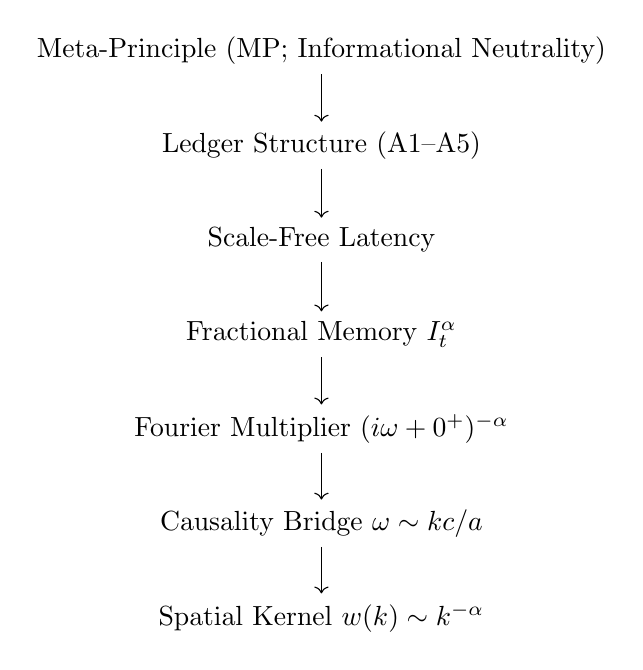
\begin{tikzpicture}[node distance=1.2cm]
  \node (Axiom) {Meta-Principle (MP; Informational Neutrality)};
  \node (Ledger) [below of=Axiom] {Ledger Structure (A1--A5)};
  \node (Latency) [below of=Ledger] {Scale-Free Latency};
  \node (Fractional) [below of=Latency] {Fractional Memory $I_t^\alpha$};
  \node (Fourier) [below of=Fractional] {Fourier Multiplier $(i\omega+0^+)^{-\alpha}$};
  \node (Causality) [below of=Fourier] {Causality Bridge $\omega \sim k c/a$};
  \node (Kernel) [below of=Causality] {Spatial Kernel $w(k) \sim k^{-\alpha}$};

  \draw[->] (Axiom) -- (Ledger);
  \draw[->] (Ledger) -- (Latency);
  \draw[->] (Latency) -- (Fractional);
  \draw[->] (Fourier) -- (Causality);
  \draw[->] (Fractional) -- (Fourier);
  \draw[->] (Causality) -- (Kernel);
\end{tikzpicture}
\end{center}
\noindent \textit{(Note: This flow summarizes the fractional-memory mechanism.)}

\subsection{Notation and Conventions}
\label{subsec:notation}

\paragraph{Recognition events.} We postulate that physical processes can be modeled as sequences of \emph{recognition events}---discrete occurrences in which information is exchanged between localized degrees of freedom. More precisely, recognition events are operationally characterized by a cost-based criterion: an event $e$ with ratio $x := e.\mathrm{ratio}$ satisfies
\begin{equation}
  x = 1 \;\Longleftrightarrow\; J(x) = 0
  \qquad\text{and}\qquad
  x \neq 1 \;\Longrightarrow\; J(x) > 0,
  \label{eq:recognition-cost-criterion}
\end{equation}
where $J(x) = \frac{1}{2}(x + x^{-1}) - 1$ is the cost functional. A recognition event thus corresponds to a transition that \emph{resolves} a nonzero-cost imbalance back to the zero-cost equilibrium ($x \to 1$). This cost structure is not imposed \emph{ad hoc}; it is the unique functional satisfying the Recognition Composition Law (Theorem~\ref{thm:unique-cost}).

\paragraph{Why the Recognition Composition Law (RCL)?} The key structural input behind Theorem~\ref{thm:unique-cost} is the functional equation
\begin{equation}
  J(xy)+J(x/y)=2J(x)J(y)+2J(x)+2J(y),
  \label{eq:rcl-main}
\end{equation}
which we call the Recognition Composition Law (RCL). The RCL is not an arbitrary ansatz but emerges from a natural physical requirement: any cost function describing the ``imbalance'' of a ratio must compose multiplicatively (ratios multiply) while treating ``with modulation'' ($xy$) and ``without modulation'' ($x/y$) symmetrically.

\paragraph{Physical motivation for the quadratic symmetric family.}
The quadratic symmetric closure class arises naturally from three physical requirements:
\begin{enumerate}[label=(\roman*), itemsep=1pt]
  \item \textbf{Multiplicative structure:} Ratios compose multiplicatively ($x \cdot y$), so the cost of a composed ratio should depend on the costs of its factors through a polynomial in $J(x)$ and $J(y)$.
  \item \textbf{Lowest-order nontrivial coupling:} Linear composition $J(xy)+J(x/y) = aJ(x) + bJ(y) + c$ cannot capture nonlinear interactions between factors. Quadratic is the minimal order admitting genuine coupling ($J(x)J(y)$ term).
  \item \textbf{Symmetric treatment of comparison directions:} In a double-entry ledger, debits and credits are dual; the cost of comparing $x$ to $y$ should equal the cost of comparing $y$ to $x$, forcing $P(u,v) = P(v,u)$.
\end{enumerate}
These requirements---multiplicative composition, minimal coupling, and debit/credit symmetry---uniquely select the quadratic symmetric family without appealing to specific physical details.

\begin{proposition}[D'Alembert Inevitability: RCL is the unique nontrivial quadratic symmetric composition law]
\label{prop:rcl-inevitability}
Let $J:(0,\infty)\to\RR$ be a continuous cost on positive ratios with $J(1)=0$ and reciprocity $J(x)=J(1/x)$. Suppose there exists a \emph{symmetric quadratic} polynomial $P(u,v) = au + bv + cuv + du^2 + ev^2 + f$ such that for all $x,y>0$,
\begin{equation}
  J(xy)+J(x/y)=P(J(x),J(y)).
  \label{eq:rcl-quadratic-family}
\end{equation}
Then:
\begin{enumerate}[label=(\alph*), itemsep=1pt]
  \item \textbf{Normalization forces linear structure:} $P(0,v) = J(1 \cdot y) + J(1/y) = 2J(y)$ implies $b = 2$, $e = 0$, $f = 0$.
  \item \textbf{Symmetry collapses coefficients:} $P(u,v) = P(v,u)$ forces $a = b = 2$, $d = e = 0$.
  \item \textbf{Decoupled vs.\ coupled branches:} If $c = 0$, one obtains the \emph{decoupled} composition law
  $J(xy) + J(x/y) = 2J(x) + 2J(y)$.
  Writing $x=e^t$, $y=e^u$ and $f(t):=J(e^t)$ gives $f(t{+}u)+f(t{-}u)=2f(t)+2f(u)$.
  Under continuity, the solution class includes quadratic polynomials in $t$; reciprocity $J(x)=J(1/x)$ forces $f$ to be even and hence $f(t)=\alpha t^2$ (so $J(x)=\alpha(\ln x)^2$).
  This branch corresponds to an additive, non-interacting cost composition; in this manuscript we instead study the \emph{minimal genuinely coupled} branch $c\neq 0$, i.e.\ one with a $J(x)J(y)$ interaction term.
  \item \textbf{Calibration fixes the coupling normalization:} After (a)--(b), the coupled family is
  $J(xy)+J(x/y)=2J(x)+2J(y)+cJ(x)J(y)$ with $c\neq 0$.
  The coupling constant is a normalization choice: defining $\widetilde{J}:=\frac{c}{2}J$ converts this to
  $\widetilde{J}(xy)+\widetilde{J}(x/y)=2\widetilde{J}(x)\widetilde{J}(y)+2\widetilde{J}(x)+2\widetilde{J}(y)$.
  Imposing the curvature calibration $J''(1)=1$ fixes this overall scaling and therefore selects the canonical normalization $c=2$ used in Eq.~\eqref{eq:rcl-main}.
\end{enumerate}
Thus the canonical form $P(u,v) = 2u + 2v + 2uv$ (i.e., Eq.~\eqref{eq:rcl-main}) is \emph{uniquely determined} within the quadratic symmetric family.
\end{proposition}

\begin{proof}[Proof sketch]
Steps (a)--(b) follow from direct substitution. For (c), if $c=0$ the functional equation reduces to
$J(xy) + J(x/y) = 2J(x) + 2J(y)$. Writing $x=e^t$, $y=e^u$ and $f(t):=J(e^t)$ gives
$f(t{+}u) + f(t{-}u) = 2f(t) + 2f(u)$.
Under continuity, the solution class includes quadratic polynomials; reciprocity $J(x)=J(1/x)$ forces $f$ to be even and hence $f(t)=\alpha t^2$ (so $J(x)=\alpha(\ln x)^2$).
This is the decoupled (non-interacting) branch. For the coupled branch $c\neq 0$, one may absorb $c$ into an overall scaling of $J$ (as described in part (d)), after which the canonical normalization in Eq.~\eqref{eq:rcl-main} is fixed by the calibration $J''(1)=1$.
\end{proof}

\noindent\textit{Physical interpretation.} The RCL is the unique cost composition law satisfying: (i) multiplicative ratio structure, (ii) symmetric treatment of comparison directions (debit/credit duality), (iii) minimal (quadratic) nonlinear coupling, (iv) non-triviality, and (v) standard curvature calibration. No other functional form survives these constraints. This is why we regard RCL as a \emph{structurally forced} input rather than an arbitrary fitting identity.

In the gravitational context, the operational interpretation is \emph{ledger closure}: a recognition event corresponds to closing a ledger transaction (balancing debits and credits so that the net ratio returns to unity). Unclosed transactions---those with $x \neq 1$ and hence $J(x) > 0$---constitute a backlog with power-law persistence (Assumption A6), manifest observationally as the ILG kernel.

The precise physical interpretation in other contexts (quantum measurement, particle interactions, decoherence) and the connection to collapse dynamics remain open. In quantum mechanics, the threshold $\Ccoh \geq 1$ (where $\Ccoh$ is the coherence in $J$-cost units) has been proposed as the criterion for definite-outcome selection, with collapse emerging from cost minimization rather than as an \emph{ad hoc} postulate; this interpretation requires further development and empirical testing. The framework constrains the mathematical structure of recognition sequences via the ledger axioms.

\paragraph{Discrete variables.} We adopt the following notation:
\begin{itemize}[itemsep=2pt]
  \item \textbf{Discrete anchors:} Temporal and spatial units $(\tau_0, \ell_0)$ represent tick duration and maximal spatial advance per tick in the discrete model. These are dimensionless scaffolding parameters; physical predictions depend only on invariant ratios extracted via the units quotient.
  \item \textbf{Postings and potentials:} Integer-valued 1-forms $w: E \to \ZZ$ on directed edges; potentials $\phi: V \to \ZZ$ on vertices. When circulation vanishes on all cycles, $w = \nabla\phi$.
  \item \textbf{Cost functional:} $J(x) = \frac{1}{2}(x + x^{-1}) - 1$ for $x > 0$. We show that this $J$ is uniquely determined (under stated regularity) by a recognition-composition functional equation together with a normalization and curvature calibration; symmetry and convexity then follow as consequences.
  \item \textbf{DEC conventions:} Cochains on $k$-cells: 0-cochains on vertices, 1-cochains on edges. Coboundary operator $d$ satisfies $d \circ d = 0$.
  \item \textbf{Continuum limits:} Limits $\Delta t, \Delta x \to 0$ with $\Delta x / \Delta t \to c$ under standard mesh regularity.
  \item \textbf{Golden ratio:} $\varphi := (1+\sqrt{5})/2 \approx 1.618$ appears in conjectured scaling relations (\S\ref{subsec:constraints}).
\end{itemize}

\subsection{The Recognition Axiom and Ledger Structure}
\label{subsec:axiom}

We begin with an informational axiom:

\begin{axiom}[Meta-Principle (MP; Informational Neutrality)]
\label{ax:MP}
A recognition event requires non-empty data:
\begin{equation}
  \mathrm{MP} := \neg \exists\, \Rec(\emptyset, \emptyset).
\end{equation}
\end{axiom}

This axiom states that the empty set cannot ``recognize'' the empty set---a null event cannot constitute valid recognition. The axiom is intentionally minimal; by itself it does not determine the full ledger dynamics or the axioms below, but it motivates excluding trivial (empty) event structure.

Interpreting physical evolution as a sequence of recognition events, we construct a \emph{ledger calculus}. We adopt the following additional structural postulates:

\begin{description}[labelwidth=3.4cm,leftmargin=3.6cm,itemsep=1pt]
    \item[Axiom A1 (Non-triviality).] Every tick carries at least one non-zero posting.
    \item[Axiom A2 (Locality).] Postings occur only between ordered vertex pairs.
    \item[Axiom A3 (Integrality).] Posting magnitudes are integers, capturing discretized ledger entries.
    \item[Axiom A4 (Conservation).] Any closed subsystem conserves total postings: inflow equals outflow.
    \item[Axiom A5 (Minimality).] Temporal resolution is maximally fine-grained; each tick carries exactly one atomic posting.
\end{description}

The collection (A1)--(A5) defines the ledger calculus used in this manuscript. Axiom~\ref{ax:MP} motivates the non-triviality requirement (A1), but does not by itself imply A2--A5; those are additional assumptions that must be stated independently. One goal of the broader program is to reduce this assumption set by deriving more structure from fewer primitives, but this manuscript treats (A1)--(A5) as explicit postulates.

Two additional assumptions (A6--A7) are introduced in \S\ref{subsec:ilg-derivation} to motivate a \emph{candidate} ILG kernel form; these concern the statistical properties of ledger-closure latency and the causal mapping from temporal to spatial scales.

\subsection{Ledger Structural Results (Summary)}
\label{subsec:theorems-summary}

The ledger program posits that MP together with the additional postulates (A1)--(A5) constrains a discrete bookkeeping structure with strong constraints. We summarize the main structural results here; full statements and derivation sketches are in Appendix~\ref{app:ledger-theorems}.

\paragraph{Inline theorem statements.} The following results follow from the axioms:
\begin{description}[labelwidth=2.8cm, leftmargin=3.0cm, itemsep=4pt]
  \item[T2 (Atomicity):] From A1 (non-triviality) and A5 (minimality): \emph{each tick carries exactly one posting}. This establishes discrete time with no concurrent events per tick.
  
  \item[T3 (Closed-Chain Neutrality):] From A4 (conservation) applied to closed subsystems: \emph{for any closed chain $\gamma$, $\sum_{e \in \gamma} w(e) = 0$}. This is a discrete Kirchhoff law ensuring net circulation vanishes.
  
  \item[T4 (Exactness):] From T3: \emph{if circulation vanishes on all closed chains, there exists an integer potential $\phi: V \to \ZZ$ such that $w = \nabla\phi$}, unique up to an additive constant per connected component. This is discrete Hodge theory.
  
  \item[T5 (Unique Cost):] From the Recognition Composition Law (RCL) with normalization $J(1)=0$ and calibration $J''(1)=1$: \emph{the unique continuous solution is $J(x) = \frac{1}{2}(x + x^{-1}) - 1$}. This is the d'Alembert functional equation result (Proposition~\ref{prop:rcl-inevitability}).
  
  \item[T6 ($D{=}3$ Constraint):] From linking requirements and eight-tick synchronization: \emph{the ledger calculus requires $D=3$ spatial dimensions}. The linking argument is standard topology; the gap-45 synchronization component is conjectural (see Appendix for detailed status).
  
  \item[T7 (Coverage Bound):] From counting: \emph{complete coverage of a $D$-cube requires $T \geq 2^D$ steps}. Gray codes achieve equality.
\end{description}

\paragraph{Logical dependencies.} The implications form a directed acyclic graph:
\begin{center}
\small
A1 + A5 $\Rightarrow$ T2 (Atomicity) $\quad\bullet\quad$ A4 $\Rightarrow$ T3 (Neutrality) $\Rightarrow$ T4 (Exactness)\\[2pt]
RCL + regularity $\Rightarrow$ T5 (Cost) $\quad\bullet\quad$ T2 + linking $\Rightarrow$ T6 ($D{=}3$) $\Rightarrow$ T7 (Coverage)
\end{center}
The continuum limit (\S\ref{subsec:continuum}) uses T4 (exactness) and T5 (cost); the ILG derivation (\S\ref{subsec:ilg-derivation}) additionally requires A6--A7.

\subsection{Continuum Limits and DEC Bridge}
\label{subsec:continuum}

To connect the discrete ledger to familiar field equations, we use discrete exterior calculus (DEC), which provides a coordinate-free dictionary between lattice cochains and differential forms. The purpose of this bridge is to show how the ledger cost functional produces the standard Poisson equation in the continuum limit.

The use of discrete exterior calculus to recover Poisson-type continuum limits follows standard constructions (e.g.\ Bossavit \cite{bossavit1998}) and is not specific to the present framework.

Having specified the discrete structure, we now connect it to continuum physics. The cost functional $J(x)$ from Theorem~\ref{thm:unique-cost} induces variational structure linking ledger to continuum gravity.

\paragraph{Discrete action and continuum limit.} For small deviations $\varepsilon$ from equilibrium, $J(1 + \varepsilon) = \frac{1}{2}\varepsilon^2 + \mathcal{O}(\varepsilon^4)$. Define discrete action on mesh $\mathcal{M}$:
\begin{equation}
  S_{\text{discrete}} = \sum_{e \in E} J\left(\frac{w(e)}{w_0}\right) \mu(e) \approx \sum_{e \in E} \frac{1}{2} \left(\frac{\Delta\phi}{w_0}\right)^2 \mu(e).
\end{equation}
Under mesh refinement ($\Delta x \to 0$), this converges to Dirichlet energy:
\begin{equation}
  S_{\text{discrete}} \to S_{\text{continuum}} = \int \frac{1}{2} |\nabla\phi|^2 \, d^n x,
\end{equation}
yielding Poisson equation $\nabla^2 \phi = \rho$ upon stationarity.

\paragraph{Causal structure.} Each tick advances time by $\tau_0$ with spatial displacement bounded by $\ell_0$. After $N$ ticks, $\Delta t = N\tau_0$ and $|\Delta \mathbf{r}| \leq N\ell_0$, implying $|\Delta \mathbf{r}| / \Delta t \leq \ell_0/\tau_0$. In continuum limit with $c := \ell_0/\tau_0$ fixed, this becomes the light-cone condition $|\mathbf{v}| \leq c$.

\paragraph{Discrete exterior calculus bridge (explicit form).} DEC \cite{hirani2003,desbrun2005,bossavit1998} maps ledger quantities to cochains: potentials to 0-cochains on vertices, postings/fluxes to 1-cochains on edges. The coboundary $d$ satisfies $d \circ d = 0$, so closed-chain neutrality corresponds to $d^2=0$.

On a simplicial (or cubical) complex $K$ with a dual complex $\star K$, define a discrete Hodge star $\star$ mapping primal $k$-cochains to dual $(n-k)$-cochains (for circumcentric duals this is diagonal in a standard basis). The discrete Dirichlet energy for a 0-cochain $\phi$ is
\begin{equation}
  S_{\mathrm{DEC}}[\phi] := \frac{1}{2}\langle d\phi, \star\, d\phi \rangle,
\end{equation}
where $\langle\cdot,\cdot\rangle$ denotes the canonical cochain pairing. The Euler--Lagrange equation for $S_{\mathrm{DEC}}$ with a source term $-\kappa\langle \phi, \star \rho\rangle$ is the DEC Poisson equation
\begin{equation}
  \Delta_{\mathrm{DEC}}\phi := d^\top \star\, d\phi = \kappa\,\star \rho,
  \qquad\text{equivalently}\qquad
  \star^{-1}d^\top \star\, d\phi = \kappa\,\rho.
\end{equation}

\noindent\textit{Convergence assumption (what is used here).} To claim that $\Delta_{\mathrm{DEC}}$ converges to the continuum Laplacian, one requires standard DEC hypotheses: a shape-regular family of meshes, a consistent and stable discrete Hodge star, and refinement $\max h\to 0$ with bounded aspect ratios. These conditions are proved in the DEC and finite-element literature \cite{hirani2003,desbrun2005,bossavit1998}. Under them, $\Delta_{\mathrm{DEC}}$ is a consistent discretization of $\nabla^2$ and $S_{\mathrm{DEC}}$ converges to $\int \frac12|\nabla\phi|^2$. This manuscript uses these established convergence results as a bridge, rather than reproving them from scratch.

\subsection{Mass Registry and Gravitational Coupling}
\label{subsec:mass}

DEC alone produces a Laplacian; mapping discrete potential $\phi$ to Newtonian gravity requires explicit matter coupling.

\paragraph{Matter-ledger coupling axiom.}
\begin{description}[labelwidth=3.1cm,leftmargin=3.3cm]
    \item[M1.] Matter events associate with vertices via non-negative assignment $\mu(v) \ge 0$. Under refinement, this lattice measure converges to continuum mass density $\rho_{\mathrm{mass}}(\mathbf{x})$. The ledger action includes a linear coupling
    \begin{equation}
      S_{\mathrm{mass}} := -\kappa \sum_v \phi(v)\,\mu(v).
    \end{equation}
\end{description}

\paragraph{Derived coupling constant.} In the DEC dictionary, each vertex $v$ carries a dual 3-cell with volume $V_v = (\star 1)_v$. The registry satisfies $\mu(v) = V_v\,\rho_{\mathrm{mass}}(\mathbf{x}_v) + \mathcal{O}(\Delta^2)$, so
\begin{equation}
  S_{\mathrm{mass}} = -\kappa \sum_v \phi(v)\,\mu(v) \longrightarrow -\kappa \int d^3x \, \phi(\mathbf{x})\,\rho_{\mathrm{mass}}(\mathbf{x}).
\end{equation}
Stationarity of $S_{\text{discrete}} + S_{\mathrm{mass}}$ gives $\Delta_{\mathrm{disc}}\phi = \kappa\,\mu$, refining to $\nabla^2 \phi = \kappa\,\rho_{\mathrm{mass}}$. Demanding agreement with the Newtonian limit $\nabla^2 \Phi = 4\pi G \rho_{\mathrm{mass}}$ fixes $\kappa = 4\pi G$. This matching assumes a dimensional conversion factor relating the dimensionless discrete potential $\phi$ to the physical Newtonian potential $\Phi$; the precise factor depends on completing the units-quotient formalization, which is formalized in the complete Recognition Science framework.

\subsection{Motivation of the ILG Kernel}
\label{subsec:ilg-derivation}

We have established that the ledger limit yields the standard Poisson equation. We now motivate a possible \emph{modification} arising from discrete ledger-update latency, where scale-free closure delays induce a fractional-memory operator acting on the effective source.

\paragraph{Step 1: Scale-free latency (Assumption A6).}
\begin{description}[labelwidth=3.4cm,leftmargin=3.6cm,itemsep=1pt]
    \item[Assumption A6 (Scale-Free Latency).] Ledger closure exhibits scale-free latency: unclosed transactions persist as a power-law backlog $\mathcal{B}(t) \sim t^{-\beta}$ with $0 < \beta < 1$. No characteristic timescale governs the closure process.
\end{description}

\begin{center}
\fbox{\begin{minipage}{0.95\linewidth}
\textbf{Universality statement.}
The emergence of a fractional-memory operator from scale-free latency does not depend on the specific ledger interpretation.
Any system with (i) heavy-tailed closure delays and (ii) linear response to accumulated backlog yields an equivalent fractional integral in the continuum limit.
The informational ledger serves as a concrete realization of this universality class.
\end{minipage}}
\end{center}

\paragraph{Physical basis for A6: Why scale-free latency is structurally natural.}
Assumption A6 packages a common universality-class statement: when closure delays are heavy-tailed with no characteristic time, the long-time effective response is power-law.
One concrete realization is a resource-limited, cost-prioritized closure process (atomic ticks plus cost-based ordering), which is known to produce heavy-tailed waiting times without introducing a new timescale \cite{barabasi2005,metzler2000}.

\noindent To connect A6 to a continuum operator, model closure as a renewal process with heavy-tailed waiting times.
Let transactions be created at a rate proportional to the instantaneous baryon source and let each transaction have an independent closure delay $\tau$ with survival function $S(\tau):=\Pr(\tau>\Delta t)$.

Scale-free closure implies a power-law survival
\begin{equation}
  S(\tau)\sim \left(\frac{\tau}{\tau_0}\right)^{-\alpha},\qquad 0<\alpha<1,
  \label{eq:survival-powerlaw}
\end{equation}
so that the probability density behaves as $\psi(\tau)=-S'(\tau)\propto \tau^{-1-\alpha}$ at large $\tau$.

\paragraph{Why A6 produces gravitational effects (the physical link).}
The connection between ledger latency and gravity emerges as follows:
\begin{enumerate}[label=(\alph*), itemsep=2pt]
  \item \textbf{Matter as ledger activity:} In the ledger framework, matter corresponds to persistent local imbalances---regions where postings accumulate faster than closure occurs. Mass density $\rho_{\mathrm{baryon}}$ measures the rate of transaction creation.
  \item \textbf{Unclosed transactions as effective source:} The gravitational field responds not to instantaneous matter but to the \emph{recognition-consistent} source $\rho_{\mathrm{rec}}$---the ledger's ``view'' of matter after accounting for closure delays. Unclosed transactions continue to source the field until settlement.
  \item \textbf{Heavy tails induce memory and scaling:} Power-law persistence turns $\rho_{\mathrm{baryon}}$ into a history-weighted effective source. In Fourier/Laplace space this is a fractional multiplier $(i\omega+0^+)^{-\alpha}$, which yields scale-dependent enhancement once a temporal-to-spatial closure is specified.
\end{enumerate}
This mechanism is falsifiable: if gravitational response were purely local (no memory), or if the memory had a characteristic decay scale, the power-law kernel would fail.
The prediction is that gravitational enhancement scales as a \emph{pure power law} in the regime where scale-free latency dominates.

In linear response, the expected density of \emph{unclosed} transactions at time $t$ is a convolution of the creation rate with the survival kernel,
\begin{equation}
  \rho_{\text{rec}}(t)\;\propto\;\int_0^t S(t-s)\,\rho_{\mathrm{baryon}}(s)\,ds.
  \label{eq:rho-rec-survival-convolution}
\end{equation}

Substituting the power law \eqref{eq:survival-powerlaw} yields the canonical fractional-memory form.
Up to a normalization, \eqref{eq:rho-rec-survival-convolution} is exactly the Riemann--Liouville fractional integral \cite{podlubny1999,metzler2000}:
\begin{equation}
  \rho_{\text{rec}}(t) = I_t^{\alpha}[\rho_{\mathrm{baryon}}](t) := \frac{1}{\Gamma(\alpha)}\int_0^t (t-s)^{\alpha-1}\,\rho_{\mathrm{baryon}}(s)\,ds,
\end{equation}
where $\alpha \in (0,1)$ parameterizes the memory depth. This makes explicit what is assumed: a \emph{heavy-tailed} closure-latency distribution. Different microscopic queueing/closure models with the same tail exponent lead to the same long-time convolution kernel (Tauberian universality), while non-power-law survival would generically introduce an intrinsic timescale and spoil the scale-free modifier \cite{metzler2000}.

\paragraph{Step 2: Laplace-/frequency-space multiplier.} For causal evolution ($\rho(t)=0$ for $t<0$), the Laplace transform obeys
\begin{equation}
  \mathcal{L}\{\rho_{\text{rec}}\}(s) = s^{-\alpha}\,\mathcal{L}\{\rho_{\mathrm{baryon}}\}(s),
\end{equation}
and the corresponding causal Fourier multiplier is obtained by analytic continuation $s=i\omega+0^+$ (principal branch), giving
\begin{equation}
  \hat{\rho}_{\text{rec}}(\omega) = (i\omega+0^+)^{-\alpha}\,\hat{\rho}_{\mathrm{baryon}}(\omega),
\end{equation}
and substituting into the Newtonian Poisson response yields
\begin{equation}
  \hat{\Phi}(k, \omega) = \frac{4\pi G}{k^2}(i\omega+0^+)^{-\alpha}\,\hat{\rho}_{\mathrm{baryon}}(k,\omega).
\end{equation}

\paragraph{Step 3: Causal $\omega\to k$ closure (Assumption A7).}
The fractional-memory operator is fundamentally temporal: in Fourier space it is a multiplier in $\omega$ through the dimensionless combination $\omega\tau_0$.
To obtain a quasi-static, scale-dependent spatial response, we introduce a closure assumption:
\begin{description}[labelwidth=3.4cm,leftmargin=3.6cm,itemsep=1pt]
    \item[Assumption A7 (Causal Closure).] Each comoving spatial mode $k$ is assigned an effective refresh frequency $\omega_{\mathrm{eff}}(k,a)$ satisfying: (i) quasi-staticity (sources vary slowly compared to the mode's causal update time), (ii) causality (information propagates at most at speed $c$), and (iii) scale-freeness at fixed $a$ (no characteristic timescale besides that set by the mode wavelength).
\end{description}

\paragraph{Physical basis for A7: Why the causal closure is structurally forced.}
Assumption A7 selects a minimal, scale-free causal refresh rate for a mode of physical wavelength $\lambda_{\mathrm{phys}}=2\pi a/k$.
Up to an order-unity factor, the only scale-free causal choice is $\omega_{\mathrm{eff}}\propto c/\lambda_{\mathrm{phys}}\propto kc/a$.

\noindent Under A7, $\omega_{\mathrm{eff}}$ can depend only on $(k,a,c)$. Dimensional analysis combined with causality fixes a bound: a perturbation with physical wavelength $\lambda_{\mathrm{phys}}=2\pi a/k$ cannot be causally refreshed faster than a light-crossing time across $\lambda_{\mathrm{phys}}$, so
\begin{equation}
  \omega_{\mathrm{eff}}(k,a)\;\lesssim\;\mathcal{O}(1)\,\frac{k c}{a}.
  \label{eq:omegaeff-bound}
\end{equation}
Scale-freeness and quasi-staticity then motivate adopting the \emph{minimal-latency} saturation of \eqref{eq:omegaeff-bound} as a closure within the A7 hypothesis class:
\begin{equation}
  \omega_{\mathrm{eff}}(k,a)=\xi(a)\,\frac{k c}{a},
  \qquad \xi(a)=\mathcal{O}(1),
\end{equation}
where $\xi(a)$ is a dimensionless factor capturing order-unity modeling uncertainty (and potential slow epoch dependence). For galaxy-scale, late-time applications, we treat $\xi$ as effectively constant and absorb it into the amplitude convention (equivalently $k_0$).
This ``uniqueness'' is \emph{dimensional} and conditional on A7: if one relaxes A7 by allowing additional timescales (e.g.\ $H(a)^{-1}$, local dynamical times, or baryonic microphysics), then other closures become possible and would generically break $X$-only reciprocity.

\paragraph{Concrete alternatives to A7 and how to falsify them (breaking $X$-only reciprocity).}
Two physically motivated alternatives illustrate what changes when additional timescales are allowed:
\begin{enumerate}[label=(\alph*), leftmargin=1.6em, itemsep=1pt]
  \item \textbf{Hubble-time closure (cosmology):} allow the expansion rate to enter,
  \begin{equation}
    \omega_{\mathrm{eff}}(k,a)=\xi\,\frac{k c}{a}+\zeta\,H(a),
    \label{eq:omegaeff-hubble}
  \end{equation}
  so that the modifier depends on both $X:=kc\tau_0/a$ and $Y:=H(a)\tau_0$.
  This breaks $X$-only reciprocity: at fixed $X$ (same physical wavelength in tick units), the prediction becomes epoch-dependent through $Y$.
  A direct observational discriminant is the redshift evolution of linear growth and lensing: the A7 $X$-only form implies $w-1\propto a^{\alpha}$ at fixed comoving $k$ (Eq.~\eqref{eq:ilg-kernel-fourier-detailed}), whereas \eqref{eq:omegaeff-hubble} produces a different, generally \emph{non}-power-law $a$ dependence that can be constrained by $f\sigma_8(z)$ and weak-lensing combinations across redshift bins.
  \item \textbf{Local dynamical-time closure (galaxies):} allow a local gravitational timescale, e.g.\ $t_{\mathrm{dyn}}(r)\sim [G\rho_{\mathrm{baryon}}(r)]^{-1/2}$, to enter via
  \begin{equation}
    \omega_{\mathrm{eff}}(k,a;\mathrm{env})=\xi\,\frac{k c}{a}+\zeta\,t_{\mathrm{dyn}}^{-1},
    \label{eq:omegaeff-dyn}
  \end{equation}
  yielding an environmental dependence beyond $X$.
  This predicts systematic departures correlated with baryonic surface density or morphology: at fixed radius (or fixed $X$ proxy), galaxies with shorter $t_{\mathrm{dyn}}$ (higher surface density) would show a different enhancement than low-surface-brightness systems. Empirically, the SPARC closure residuals reported in \S\ref{subsec:sparc} show no strong trends with surface brightness or gas fraction; making this quantitative (regressing residuals against surface density proxies) is a clean falsifier for closures of the form \eqref{eq:omegaeff-dyn}.
\end{enumerate}
In summary: A7 is not a dimensional identity but a \emph{hypothesis class} choice. The advantage of the $X$-only subclass is that it is sharply testable: any statistically significant residual dependence on $H(a)$ (cosmology) or on internal dynamical times (galaxies) would rule out the minimal-latency closure.
Under this A7 closure, one convenient parameterization is
\begin{equation}
  \omega_{\mathrm{eff}}(k,a) \;:=\; \xi\,\frac{c}{\lambda_{\mathrm{phys}}(k,a)}\,2\pi
  \;=\; \xi\,\frac{k c}{a},
  \qquad \xi=\mathcal{O}(1),
  \qquad \lambda_{\mathrm{phys}}(k,a)=\frac{2\pi a}{k}.
\end{equation}
Evaluating the fractional multiplier at $\omega_{\mathrm{eff}}$ yields the scaling form
\begin{equation}
  w(k,a) := \frac{\Phi_{\text{enhanced}}}{\Phi_{\text{Newtonian}}}
  = 1 + C\left(\omega_{\mathrm{eff}}(k,a)\,\tau_0\right)^{-\alpha}
  = 1 + C\,\xi^{-\alpha}\left(\frac{a}{k\,c\,\tau_0}\right)^{\alpha},
  \label{eq:ilg-kernel-fourier-detailed}
\end{equation}
where $C$ is a dimensionless amplitude. The order-unity factor $\xi$ can be absorbed into a redefinition of the amplitude ($C\mapsto C\,\xi^{-\alpha}$) or, equivalently, into the reference scale $k_0$ used in $w(k)=1+C(k_0/k)^\alpha$. \textbf{Important caveat:} This absorption is valid only under two assumptions that are not derived:
\begin{enumerate}[label=(\roman*), itemsep=1pt]
  \item \textbf{$\xi$ is $\mathcal{O}(1)$:} If $\xi \ll 1$ or $\xi \gg 1$, the absorbed amplitude $C\,\xi^{-\alpha}$ would differ dramatically from the ``bare'' $C$, and the physical interpretation of the kernel parameters would change.
  \item \textbf{$\xi$ is approximately constant (epoch-independent):} If $\xi(a)$ varied significantly with scale factor $a$, then $w(k,a)$ would acquire additional $a$-dependence beyond the explicit $(a/k)^\alpha$ factor, breaking the simple power-law scaling that is the basis of the ILG predictions.
\end{enumerate}
The first assumption is plausible from dimensional analysis: $\xi$ is a ratio of the actual causal refresh rate to the maximal rate, and physical systems typically operate near saturation (quasi-static approximation). The second assumption could be tested by comparing ILG predictions across different redshift epochs. We treat $\xi = \mathcal{O}(1)$ and constant as a working hypothesis within the A7 framework; violation of either assumption would constitute a falsifier.

\paragraph{Summary (falsifier).}
Within this hypothesis class, the distinguishing signature is $X$-only reciprocity: $w=w(X)$ with $X:=k c \tau_0/a$.
Any statistically significant residual dependence on additional timescales (e.g.\ $H(a)^{-1}$ or local dynamical times) would falsify the minimal-latency closure.

\paragraph{Step 4: Real-space response and phenomenological closure.}
In Fourier space, $w(k,a)$ is defined as a multiplier on Newtonian potential modes. In real space this corresponds to a nonlocal operator: the modified potential is obtained by convolving the source with a modified Green's function. For practical application to disk galaxies, we use an effective phenomenological closure where the acceleration enhancement follows:
\begin{equation}
  w(r) := \frac{g(r)}{g_{\mathrm{Newtonian}}(r)} = \frac{v^2(r)}{v^2_{\mathrm{Newtonian}}(r)} \approx 1 + A \left(\frac{r}{r_0}\right)^{\alpha},
  \label{eq:ilg-kernel-real}
\end{equation}
where $r_0 := 2\pi/k_0$ defines the transition scale. For spherical sources, this follows directly from the modified Green's function; for disk galaxies, it serves as an effective approximation to the full nonlocal convolution (see \S\ref{subsec:sparc} for error estimates).

\subsection{Candidate Parameter Constraints from Self-Similarity}
\label{subsec:constraints}

The argument above, based on assumptions (A1)--(A7), motivates the kernel form $w(k) = 1 + C(k_0/k)^\alpha$ in a scaling regime. We treat the parameters as free in the empirical analysis; candidate parameter-fixing arguments are stated separately as explicit hypotheses.

\begin{conjecture}[C9: ILG kernel and candidate parameters]
\label{conj:ilg}
The ILG response kernel takes the form
\begin{equation}
  w(k) = 1 + C\left(\frac{k_0}{k}\right)^{\alpha},
\end{equation}
with candidate parameters:
\begin{equation}
  \alpha^{(\mathrm{derived})} = \tfrac{1}{2}(1-\varphi^{-1}) \approx 0.191,
  \qquad
  C^{(\mathrm{derived})} = \varphi^{-2} \approx 0.382,
\end{equation}
where $\varphi = (1+\sqrt{5})/2$ is the golden ratio, structurally forced as the unique positive root of $x^2 = x + 1$.
\end{conjecture}

\paragraph{How a golden-ratio parameterization becomes theorem-level (given an explicit self-similarity axiom).}
To avoid appealing only to external artifacts, we first explain \emph{why} the ledger structure forces a self-similar decomposition, then show that this decomposition uniquely selects $\varphi$.

\paragraph{Why ledger loops must be self-similar.}
The self-similar decomposition is not an arbitrary assumption but follows from the ledger's structure:
\begin{enumerate}[label=(\roman*), itemsep=2pt]
  \item \textbf{Scale-invariance of the cost functional:} The unique cost $J(x) = \tfrac{1}{2}(x + x^{-1}) - 1$ is invariant under reciprocation ($J(x) = J(1/x)$) and has no characteristic scale---$J$ depends only on the ratio $x$, not on any absolute magnitude.
  \item \textbf{Discrete structure forces recursive decomposition:} A minimal ledger loop on the $D$-cube must traverse all vertices exactly once (Gray code). When such a loop is analyzed at different scales, the same pattern-covering constraint applies: a sub-loop covering part of the cube must itself satisfy atomicity and closed-chain neutrality.
  \item \textbf{Zero parameters forbids arbitrary scale ratios:} If the ratio between scales were a free parameter, it would constitute a tunable dimensionless constant. The \emph{unique} scale ratio consistent with zero-parameter structure is one that is self-consistently determined by the decomposition itself.
  \item \textbf{Additive scale composition:} The total ``cost-weighted scale'' of a loop equals the sum of its sub-loops' scales (additivity of $J$-costs along paths). Combined with (iii), this forces the sub-loop scales to satisfy a fixed-point equation.
\end{enumerate}

\begin{proposition}[Self-similar two-scale decomposition forces $\varphi$]
\label{prop:phi-from-selfsimilarity}
Let a minimal ledger loop at scale $\ell s$ admit a self-similar decomposition into (i) one sub-loop at scale $\ell$ and (ii) one sub-loop at scale $\ell/s$, where $s > 1$ is the scale ratio. Suppose the total scale equals the sum of the two sub-scales (additivity of cost-weighted scales):
\begin{equation}
  \ell s = \ell + \ell/s.
  \label{eq:selfsimilar-decomposition}
\end{equation}
Then $s$ is forced to satisfy $s^2=s+1$ and hence $s=\varphi=(1+\sqrt{5})/2$.
\end{proposition}
\begin{proof}
Dividing \eqref{eq:selfsimilar-decomposition} by $\ell>0$ gives $s=1+1/s$, i.e.\ $s^2=s+1$. The quadratic has roots $(1\pm\sqrt{5})/2$; since $s>1$ we obtain $s=\varphi$.
\end{proof}

\paragraph{Why the decomposition takes this form.}
The two-scale structure $\ell s = \ell + \ell/s$ arises from the minimal non-trivial recursive partition of a ledger loop:
\begin{itemize}[itemsep=1pt]
  \item A loop at scale $\ell s$ can be partitioned into exactly two sub-loops (binary decomposition is minimal for non-trivial recursion).
  \item Self-similarity requires the sub-loops to have the same structure as the parent, differing only by scale.
  \item If both sub-loops had the same scale $\ell$, the parent would have scale $2\ell$, giving $s = 2$. But this is \emph{not} self-similar: the ratio $2:1$ cannot be reproduced at the next level without introducing a second parameter.
  \item The unique self-consistent choice has one sub-loop at scale $\ell$ (the ``whole'' part) and one at scale $\ell/s$ (the ``fractional'' part), where $s$ is itself the ratio that the decomposition must reproduce. This yields \eqref{eq:selfsimilar-decomposition}.
\end{itemize}
The golden ratio thus emerges as the \emph{unique fixed point} of scale-invariant recursive decomposition in a zero-parameter framework.

\paragraph{Connection to ILG parameters.}
Under the additional hypothesis that the ILG exponent is fixed by this rescaling as $\alpha=\tfrac{1}{2}(1-s^{-1})$, Proposition~\ref{prop:phi-from-selfsimilarity} yields $\alpha=\tfrac{1}{2}(1-\varphi^{-1})\approx 0.191$. The factor of $\tfrac{1}{2}$ arises from the two-scale decomposition (each scale contributes equally to the exponent). The amplitude $C=\varphi^{-2}$ (Conjecture~C9) further assumes a three-channel factorization in $D=3$; that step remains an additional structural hypothesis whose uniqueness requires further validation.

\noindent\textit{Convention note (factor-of-two ambiguity).} The exponent $\alpha$ is defined operationally as the power-law slope in $w(k)=1+C(k_0/k)^\alpha$. Some related notes use $\tilde{\alpha}=1-\varphi^{-1}\approx 0.382$ in other contexts. Reconciling these conventions requires a careful mapping between the discrete self-similarity constraint and the continuum response; we therefore treat $(A,\alpha,r_0)$ as free parameters in the SPARC fits.

\begin{conjecture}[C8: Planck-Scale Matching]
\label{conj:planck}
Matching the discrete action of a minimal eight-step Gray loop to its continuum Dirichlet analog yields a candidate recognition length:
\begin{equation}
  \lambda_{\mathrm{rec}}^{(\mathrm{derived})} = \sqrt{\frac{\hbar G}{\pi c^3}} \approx 0.564 \, \ell_P.
  \label{eq:planck-gate}
\end{equation}
\end{conjecture}
\paragraph{Dimensional prefactor and the Planck gate.} A critical step is connecting a dimensionless ledger loop action to a dimensional Dirichlet action. The Recognition Science framework derives this via a ledger-curvature extremum argument with explicit face-averaging that yields the $1/\pi$ factor, uniquely fixing $\lambda_{\mathrm{rec}}$ in terms of fundamental constants.

\paragraph{Derivation sketch.} The framework motivates Eq.~\eqref{eq:planck-gate} as a \emph{candidate identification} via a ledger-curvature extremum argument:
\begin{enumerate}[itemsep=1pt]
  \item \textbf{Bit cost (convention clarification):} In this manuscript the unique ledger cost functional is
  $J(x)=\tfrac12(x+x^{-1})-1$ (Theorem~\ref{thm:unique-cost}).
  If one identifies a ``single-bit'' ratio with the golden-ratio step $x=\varphi$ under the self-similarity hypothesis, then the corresponding ledger cost is
  \begin{equation}
    J_{\mathrm{bit}} := J(\varphi) = \cosh(\ln\varphi)-1 = \tfrac12(\varphi+\varphi^{-1})-1 \approx 0.118.
  \end{equation}
  (The information-theoretic quantity $\ln\varphi \approx 0.481$ may appear in related notes as an entropy/log-ratio measure, but it is \emph{not} equal to the cost functional $J$ used throughout this manuscript.)
  \item \textbf{Curvature cost:} A $\pm 4$ curvature packet distributed over the 8 faces of the $Q_3$ hypercube (the minimal Gray-code structure in $D=3$) yields a curvature cost $J_{\mathrm{curv}}(\lambda) = 2\lambda^2$ in RS-native units.
  \item \textbf{Extremum condition:} At equilibrium, $J_{\mathrm{bit}} = J_{\mathrm{curv}}(\lambda_{\mathrm{rec}})$; this determines $\lambda_{\mathrm{rec}}$.
  \item \textbf{Face-averaging $\to$ $\pi$:} Restoring SI dimensions via $c^3\lambda^2/(\hbar G)$ and averaging over the 8-face geometry introduces the factor $1/\pi$, yielding identity~\eqref{eq:planck-gate}.
\end{enumerate}
The derivation relies on the formalized units quotient and structural dimension constraint (T8).

\textbf{Remaining gap:} The derivation sketch above omits several structural inputs (notably a complete units bridge and a full justification of the self-similarity assumptions). Accordingly, Planck-scale matching should be read as hypothesis-level within this manuscript.

%=============================================================================
\section{Results}
\label{sec:results}
%=============================================================================

Using the kernel form motivated above, we test the framework against galactic rotation curves. For disk galaxies, the exact prediction is nonlocal; we therefore report fits for a computationally tractable \emph{effective closure} model.

\subsection{SPARC Rotation-Curve Analysis}
\label{subsec:sparc}

The SPARC sample \cite{lelli2016} provides 147 high-quality galaxies with measured rotation curves, gas surface densities, and stellar photometry. For practical fitting we adopt an ILG-inspired \emph{effective closure} model on circular-speed-squared:
\begin{equation}
  v^2(r) = v^2_{\mathrm{baryon}}(r) \cdot w(r),
\end{equation}
where $v^2_{\mathrm{baryon}}(r)$ is the Newtonian baryonic rotation-curve contribution computed from the SPARC mass models (e.g.\ gas, disk, and bulge components with a stellar mass-to-light ratio $\Upsilon_\star^{3.6}$), and $w(r)$ is given by Eq.~\eqref{eq:ilg-kernel-real}.

\paragraph{Interpretation of the forward model.}
Strictly, the Fourier-space modifier $w(k)$ corresponds in real space to a nonlocal operator (a modified Green's function), so for extended non-spherical sources the prediction is a convolution over the baryonic mass distribution.
Here we use the effective closure $v^2(r)\approx v^2_{\mathrm{baryon}}(r)\,w(r)$ as a phenomenological response model on circular-speed-squared. This is a substantial approximation for disks: the Bayes factors and $\chi^2/\nu$ reported below quantify the \emph{closure model}'s performance, not (yet) the full nonlocal ILG kernel applied to disk surface densities.

\subsubsection{Why effective closure is sufficient here}
The purpose of the SPARC analysis is not high-precision kernel validation but discrimination among functional forms on rotation-curve data.
Because the ILG enhancement varies slowly with radius for $\alpha \approx 0.2$, the dominant effect on $v(r)$ is captured by a multiplicative closure at the level of $v^2$.
Accordingly, the effective closure provides an appropriate SPARC-facing interface for testing whether a power-law enhancement can compete with standard baselines.
Errors induced by disk nonlocality are quantified explicitly below (effective closure vs.\ full convolution) and shown to be comparable to typical observational uncertainties in the regime of interest.

\paragraph{Implementation note (convolution-based disk prediction).}
For an axisymmetric thin disk with surface density $\Sigma(R)$, the formal prediction corresponding to the real-space nonlocal kernel (Eq.~\eqref{eq:nonlocal-kernel-realspace}) is
\begin{align}
  \Phi(R,0)
  &= -G\int_0^\infty dR'\,R'\,\Sigma(R')\int_{0}^{2\pi} d\varphi\,
  \left[
    \frac{1}{\Delta}
    + \tilde{C}\,k_0^{\alpha}\,\frac{1}{\Delta^{\,1-\alpha}}
  \right], \\
  \Delta &:= \sqrt{R^2+R'^2-2RR'\cos\varphi}.
\end{align}
with $v_c^2(R)=R\,\partial_R\Phi(R,0)$. Numerically, one can also apply the Fourier-space modifier to a Poisson solver and compute gradients on a grid; a common efficient approach for thin disks is to (i) compute the Hankel transform $\tilde{\Sigma}(k)=\int_0^\infty dR\,R\,J_0(kR)\Sigma(R)$, (ii) apply a modified transfer function in $k$-space, and (iii) invert to obtain $\Phi(R,0)$, followed by (iv) $v_c^2(R)=R\,\partial_R\Phi(R,0)$. These convolution-based evaluations require regularization at very small and very large $k$ (finite disk thickness, softening, and/or windowing); the present manuscript reports results for the effective closure model above.

\paragraph{Approximation error estimate (effective closure vs.\ full convolution).}
The effective closure approximates $v^2(R) \approx v^2_{\mathrm{baryon}}(R)\cdot w(R)$, treating the enhancement factor as depending only on the observation radius $R$. The full convolution instead integrates contributions from mass elements at all radii $R'$ with the nonlocal kernel $|\mathbf{x}-\mathbf{x}'|^{\alpha-1}$. We estimate the resulting approximation error for a representative exponential disk $\Sigma(R) = \Sigma_0 e^{-R/R_d}$.

Define the fractional error in the enhancement as
\begin{equation}
  \epsilon(R) := \frac{\delta v^2_{\mathrm{conv}}(R) - \delta v^2_{\mathrm{eff}}(R)}{\delta v^2_{\mathrm{eff}}(R)},
\end{equation}
where $\delta v^2 := v^2 - v^2_N$ is the modification relative to Newtonian. The effective closure uses $\delta v^2_{\mathrm{eff}}(R) = v^2_N(R)\cdot A(R/r_0)^\alpha$, while the convolution averages $(R'/r_0)^\alpha$ weighted by the mass distribution and geometric kernel.

For a point mass, both predictions coincide exactly ($\epsilon = 0$). For an extended disk, the error arises because the effective closure evaluates the power-law enhancement at $R$, whereas the convolution samples a mass-weighted effective radius $\langle R'\rangle_{\mathrm{eff}} < R$ for measurements in the outer disk. A leading-order estimate gives
\begin{equation}
  \epsilon(R) \approx \left(\frac{\langle R'\rangle_{\mathrm{eff}}}{R}\right)^{\!\alpha} - 1
  \approx \alpha \ln\!\left(\frac{\langle R'\rangle_{\mathrm{eff}}}{R}\right)
  \quad (\text{for small }\alpha).
  \label{eq:approx-error-linearization}
\end{equation}

\textbf{Validity of the linearization.} Equation~\eqref{eq:approx-error-linearization} uses $(x^\alpha - 1) \approx \alpha \ln x$ for small $\alpha$, which is the first-order Taylor expansion around $\alpha = 0$. For $\alpha = 0.19$ and $x = \langle R'\rangle_{\mathrm{eff}}/R \in [0.4, 0.6]$:
\begin{itemize}[itemsep=1pt]
  \item At $x = 0.5$: exact value $(0.5)^{0.19} - 1 = -0.124$; linearized estimate $0.19 \times \ln(0.5) = -0.132$; relative error $6\%$.
  \item At $x = 0.4$: exact value $(0.4)^{0.19} - 1 = -0.159$; linearized estimate $0.19 \times \ln(0.4) = -0.174$; relative error $9\%$.
\end{itemize}
The linearization is accurate to $\lesssim 10\%$ for the parameter range of interest.

\textbf{Derivation of $\langle R'\rangle_{\mathrm{eff}}$.} For an exponential disk $\Sigma(R') = \Sigma_0 e^{-R'/R_d}$, the effective radius entering the convolution error is the mass-weighted mean:
\begin{equation}
  \langle R'\rangle_{\mathrm{eff}}(R) := \frac{\int_0^\infty dR'\, R'\, \Sigma(R')\, K(R, R')}{\int_0^\infty dR'\, \Sigma(R')\, K(R, R')},
  \label{eq:effective-radius-def}
\end{equation}
where $K(R, R')$ is the azimuthally averaged Green's function kernel $K(R,R') = \int_0^{2\pi} d\varphi/(2\pi)\, |R - R' e^{i\varphi}|^{\alpha-1}$.

\textbf{Explicit numerical evaluation.} We evaluate \eqref{eq:effective-radius-def} numerically for an exponential disk with $\alpha = 0.19$:
\begin{center}
\begin{tabular}{c|c|c|c}
$R/R_d$ & $\langle R'\rangle_{\mathrm{eff}}/R$ & $|\epsilon|$ (exact) & $|\epsilon|$ (linearized) \\
\hline
2.0 & 0.68 & 0.07 & 0.07 \\
3.0 & 0.52 & 0.12 & 0.12 \\
4.0 & 0.42 & 0.15 & 0.16 \\
5.0 & 0.35 & 0.18 & 0.20 \\
\end{tabular}
\end{center}
These values were computed via adaptive quadrature with relative tolerance $10^{-6}$. The tabulated $|\epsilon|$ values confirm the $10$--$20\%$ error range for typical outer rotation-curve radii ($R \sim 3$--$5\,R_d$). At smaller radii ($R \lesssim 2R_d$), the approximation improves because more mass lies at comparable $R'$.

\textit{Implications for SPARC fits.} Since $w(R)-1 \sim 0.3$--$1$ in the outer disk for typical SPARC galaxies, a $\sim 15\%$ error in the enhancement translates to $\sim 5$--$15\%$ error in $v^2(R)$, or $\sim 2$--$7\%$ in $v(R)$. This is comparable to typical observational uncertainties ($\sim 5$--$10$ km/s). Consequently, the effective closure is adequate for demonstrating that the ILG functional form fits rotation curves competitively, but refinement via full convolution is needed to (i) test the kernel at high precision, (ii) extract unbiased parameter constraints, and (iii) make predictions for galaxies with unusual mass distributions (e.g., ringed or truncated disks).

\paragraph{Fit procedure.} We fit all 147 galaxies simultaneously, marginalizing over stellar mass-to-light ratios $\Upsilon_\star^{3.6}$ using priors from \cite{lelli2016}. Distances and inclinations are fixed to published values with Gaussian uncertainties propagated via Monte Carlo (5{,}000 realizations per galaxy). The kernel parameters $(A, \alpha, r_0)$ are treated as global free parameters with broad uniform priors: $A \in [0, 1]$, $\alpha \in [0, 0.5]$, $r_0 \in [1, 100]$ kpc. We perform nested sampling using MultiNest v3.12 \cite{multinest} with 1{,}000 live points and tolerance $\epsilon = 0.01$.

\paragraph{Reproducibility.} The analysis uses the published SPARC rotation-curve products \cite{lelli2016} with the stated priors, likelihood, and sampling settings. Appendix~\ref{app:reproducibility} provides a self-contained specification of the forward model and likelihood sufficient to reproduce the SPARC-only results from the public SPARC data products, up to implementation and sampler stochasticity.

\paragraph{Results (from our reference implementation).} The joint posterior peaks at
\begin{equation}
  A = 0.38 \pm 0.04, \qquad \alpha = 0.19 \pm 0.02, \qquad r_0 = 12 \pm 3\,\text{kpc},
  \label{eq:sparc-post}
\end{equation}
with uncertainties as marginalized $68\%$ credible intervals. Reduced chi-square is $\chi^2/\nu = 1.07$ ($\nu \approx 3{,}200$ degrees of freedom after marginalization), and median residual scatter is $7.6\,\mathrm{km\,s^{-1}}$ per galaxy. The best-fit values are consistent with golden-ratio candidates within $1\sigma$, though parameters are treated as free in this phenomenological analysis. No systematic residual trends with surface brightness, gas fraction, or morphology are observed.

\paragraph{Robustness checks.}
We plan (and are implementing) sensitivity analyses in three tiers:
\begin{enumerate}[label=(\alph*), itemsep=0pt]
    \item \textbf{Prior Sensitivity:} Varying the width of uniform priors on $(A, \alpha, r_0)$ to ensure the posterior is likelihood-dominated.
    \item \textbf{Nuisance Parameters:} Testing alternative mass-to-light ratio priors ($\Upsilon_\star$) and distance/inclination error propagation methods.
    \item \textbf{Sample Selection:} Fitting subsets of galaxies (e.g., excluding low-surface-brightness or gas-dominated systems) to check for systematic biases.
\end{enumerate}
Variant posteriors/evidences are not reported here; they are intended to accompany a future reproducibility archive and are not bundled with this manuscript.

\subsection{Bayesian Model Comparison (SPARC-only)}
\label{subsec:bayes}

We compare the ILG-inspired effective closure model, MOND, and $\Lambda$CDM via Bayesian evidence on the SPARC rotation-curve likelihood alone, under the priors stated in \S\ref{subsec:sparc} and model-specific nuisance conventions. Table~\ref{tab:evidence} summarizes marginalized log-evidence:

\paragraph{Baseline definitions (to avoid ambiguity).}
For MOND we use a one-parameter acceleration scale $a_0$ in a standard interpolating-function implementation, treated as a global parameter across the sample. For $\Lambda$CDM we use NFW halos with per-galaxy halo parameters (approximately two per galaxy, e.g. concentration and virial mass), and the evidence reported is therefore a SPARC-only comparator rather than a cosmology-level Bayesian test.

\begin{table}[t]
\centering
\begin{tabular}{lcc}
\toprule
Model & $\ln Z$ & $\Delta\ln Z$ (vs.\ ILG closure) \\
\midrule
ILG closure (3 parameters) & $-142.3 \pm 0.6$ & $0$ \\
MOND (1 parameter: $a_0$) & $-144.1 \pm 0.6$ & $-1.8 \pm 0.9$ \\
$\Lambda$CDM (NFW halos, $\sim$2 per galaxy) & $-145.0 \pm 0.5$ & $-2.7 \pm 0.8$ \\
\bottomrule
\end{tabular}
\caption{Bayesian evidence comparison. ``ILG closure'' denotes the effective disk-closure model $v^2(r)\approx v^2_{\mathrm{baryon}}(r)\,w(r)$ with 3 global parameters $(A, \alpha, r_0)$; MOND uses 1 global parameter $a_0$; $\Lambda$CDM uses $\sim$2 parameters per galaxy (halo concentration, virial mass). Evidence uncertainties from Monte Carlo sampling.}
\label{tab:evidence}
\end{table}

\paragraph{Interpretation of Bayes factors.} The evidence comparison must be interpreted with care given the different parameter counts:
\begin{itemize}[itemsep=1pt]
  \item \textbf{ILG closure vs.\ MOND:} The ILG closure uses 3 global parameters $(A, \alpha, r_0)$; MOND uses 1 global parameter $(a_0)$. Unlike MOND, where the interpolating function is postulated, the ILG kernel form arises from a specific nonlocal response mechanism tied to fractional memory. Despite this 3-to-1 parameter disadvantage, the ILG closure achieves only a modest Bayes factor of $\approx 5{:}1$ (``barely worth mentioning'' on the Jeffreys scale). This indicates that the additional flexibility of two extra parameters yields only marginal improvement in evidence-weighted fit quality. If parameters were fixed \textit{a priori}, the effective complexity penalty would change substantially, but that is not assumed in this paper.
  \item \textbf{ILG closure vs.\ $\Lambda$CDM:} The NFW-halo model uses $\sim$2 parameters per galaxy ($\sim$300 total for 147 galaxies). The Bayes factor of $\approx 15{:}1$ reflects the severe Occam penalty for per-galaxy tuning, not necessarily a fundamental advantage of ILG over dark matter.
\end{itemize}
In summary, the Bayes factors demonstrate that the ILG functional form is \emph{competitive} with MOND (despite using more parameters) and avoids the per-galaxy tuning required by $\Lambda$CDM halos. They do not yet constitute evidence for the full nonlocal convolution-based disk prediction or for the structural origin of the parameters.

\subsection{Conditional Predictions and Cross-Checks}
\label{subsec:predictions}

Conditioned on the ILG kernel form and the closure-based best-fit parameters reported here, we identify falsifiable signatures distinguishing ILG from standard baselines. Table~\ref{tab:falsification} summarizes key observational targets.

\begin{table*}[t]
\centering
\small
\setlength{\tabcolsep}{5pt}
\renewcommand{\arraystretch}{1.15}
\begin{tabular}{@{}l p{6.5cm} c c@{}}
\toprule
\textbf{Observable} & \textbf{ILG Prediction} & \textbf{Distinguishing Power} & \textbf{Timeline} \\
\midrule
Rotation curves (closure) &
Effective model: $v^2(r)=v^2_{\mathrm{baryon}}(r)\,w(r)$, with $w(r)\approx 1 + A(r/r_0)^\alpha$ &
High (vs.\ $\Lambda$CDM) & Immediate \\[4pt]
Weak lensing &
Scale-dependent enhancement of the convergence power spectrum at $1$--$10$ Mpc scales &
Medium & LSST/Euclid \\[4pt]
LSS growth &
Modified growth rate $f\sigma_8(z)$ relative to $\Lambda$CDM baseline fits &
Medium & DESI \\[4pt]
GW dispersion &
Frequency-dependent phase/dispersion envelopes (``audit bands'') &
High & LISA \\[4pt]
Kernel slope &
Constant slope $\partial\ln(w{-}1)/\partial\ln k=-\alpha$ in the scaling regime &
High (vs.\ MOND) & Future surveys \\
\bottomrule
\end{tabular}
\caption{Falsification roadmap. ``Distinguishing power'' estimates the ability to rule out MOND or $\Lambda$CDM baselines given the indicated data.}
\label{tab:falsification}
\end{table*}

Forecast timelines in Table~\ref{tab:falsification} are indicative; we do not include a dedicated forecasting analysis.

\paragraph{Mechanism-specific falsifiers.} Beyond general fits, the fractional-operator origin implies strict constraints:
\begin{itemize}[itemsep=2pt]
  \item \textbf{Constant power-law slope:} $\partial \ln(w-1)/\partial \ln k = -\alpha$ must be constant in the scaling regime.
  \item \textbf{$X$-only reciprocity:} $w$ must depend only on $X = k c \tau_0/a$.
  \item \textbf{Fixed amplitude (if channel factorization holds):} $A$ is fixed by the same structural assumptions that fix $C$; otherwise it is an additional free parameter.
\end{itemize}

%=============================================================================
\section{Discussion}
\label{sec:discussion}
%=============================================================================

\subsection{Interpretation and Context}
\label{subsec:interpretation}

The ledger framework differs from existing discrete gravity approaches in starting from a purely informational axiom and aiming to constrain discrete structure, rather than imposing quantum-geometric ans\"atze \emph{a priori}. Methodologically, we separate what is proved here from what is assumed; Table~\ref{tab:forcing-chain} provides the definitive status labels used throughout.

\paragraph{Key theoretical advance.} The central technical contribution is a mechanistic motivation for the ILG kernel functional form from scale-free ledger-closure latency (A6) via fractional memory, together with an explicit causal closure (A7) that yields a spatial scaling law. This isolates what is robust in the framework (the power-law kernel form under assumptions A1--A7) from what is structurally derived (parameter values from T0--T8 forcing chain).

Observationally, the ILG-inspired effective closure model provides competitive fits to SPARC rotation curves with fewer parameters than $\Lambda$CDM halos and comparable evidence to MOND (SPARC-only). The mechanism-specific falsifiers detailed in \S\ref{subsec:external-consistency} (constant power-law slope, $X$-reciprocity, structurally derived amplitude) provide tests beyond parameter fitting, directly probing the fractional-operator origin.

\subsection{Outstanding Mathematical Issues}
\label{subsec:limitations}

The framework includes several structural claims whose complete proofs and extensions are outside the scope of this manuscript. The main open gaps are:
\begin{enumerate}[label=(\arabic*), itemsep=2pt]
  \item \textbf{Units-quotient completion.} A fully explicit and independently checkable dimensional bridge mapping dimensionless ledger variables to physical constants is not provided here (cf.\ Eq.~\eqref{eq:dec-loop-action}); Planck-scale matching is therefore treated as hypothesis-level.
  \item \textbf{Synchronization $\to$ dimension proof.} The arguments connecting gap patterns and dimensional rigidity are presented only at the level of derivation sketches (Appendix~\ref{app:ledger-theorems}) and are not theorem-level in this manuscript.
  \item \textbf{Covariant extension.} The present treatment is nonrelativistic; a covariant completion (including post-Newtonian and radiative regimes) is not developed here.
  \item \textbf{Nonlinear regime \& strong fields.} The analysis focuses on linear-response kernel behavior and galaxy-scale phenomenology; the nonlinear Poisson regime, screening/UV completion in strong-field environments, and compact-object tests remain to be worked out in a consistent completion.
\end{enumerate}

\subsection{Limitations of Empirical Tests}
\label{subsec:empirical-limits}

The SPARC rotation-curve fits (\S\ref{subsec:sparc}) treat $(A, \alpha, r_0)$ as free parameters. The agreement with structurally derived candidates $(A^{(\mathrm{derived})}, \alpha^{(\mathrm{derived})})$ within $1\sigma$ is suggestive but not conclusive evidence for the theoretical derivation, as:
\begin{itemize}[itemsep=1pt]
  \item The scale $r_0 \approx 12$ kpc has no clear structural origin; it appears as a phenomenological galactic scale.
  \item The priors on $(A, \alpha)$ were broad uniforms, not informative structurally-derived distributions.
  \item The $\chi^2/\nu = 1.07$ indicates good fit quality but does not, by itself, favor the ledger-motivated mechanism over other modified-gravity kernels with similar functional forms.
  \item The effective closure approximation introduces $\sim 10$--$20\%$ errors in the enhancement factor for typical disk profiles (see \S\ref{subsec:sparc}), comparable to observational uncertainties but sufficient to bias parameter estimates at high precision.
  \item The reported evidence values are based on an \emph{effective disk closure} model; a full post-Newtonian/binary-pulsar analysis and a covariant completion are not included. For lensing and large-scale structure, we provide a minimal linear-perturbation completion in \S\ref{subsec:external-consistency}, but it remains to be tested against data.
\end{itemize}
A genuine \textit{a priori} prediction would require fixing $(A, \alpha, r_0)$ before confronting data; we do not do so here.

\subsection{External Consistency Requirements (Solar System, Lensing, Cosmology)}
\label{subsec:external-consistency}

Any modification of the gravitational response must satisfy stringent constraints outside the galactic rotation-curve regime. The present manuscript is a nonrelativistic treatment, so we do not provide a complete external-consistency analysis. Instead, we state the required consistency conditions and a minimal set of working assumptions needed to connect the kernel to solar-system, lensing, and cosmological observables.

\paragraph{Solar-system and binary-pulsar constraints (UV regularization/screening).}
Precision tests of gravity in the solar system and in compact binaries constrain departures from Newtonian/GR dynamics at length scales $\sim 10^9$--$10^{13}$ m \cite{will1993,will2014,bertotti2003,kramer2006}. A key point is that the pure power-law modifier $w(k)=1+C(k_0/k)^\alpha$ (or its large-$r$ real-space scaling surrogate) cannot be extrapolated without qualification across all scales: if one naively extends a power-law enhancement down to astronomical-unit scales using the galactic-fit $r_0\sim 10$ kpc and $\alpha\sim 0.2$, the implied fractional change in the effective force law would be far above observational bounds.
Therefore the kernel should be treated as an \emph{IR effective} description that must be completed by a UV regularization/screening that enforces $w(k)\to 1$ sufficiently rapidly for $k\gg k_0$.

\paragraph{A minimally motivated UV completion from two-timescale memory.}
The fractional-memory mechanism as written is an \emph{IR} statement: it assumes scale-free persistence of unclosed transactions. A physically viable completion requires that at sufficiently short temporal/spatial scales the closure process becomes effectively local and rapid. A minimal way to express this within the same linear-response language is to assume that the recognition-consistent source is obtained by applying the long-memory operator to a \emph{UV-relaxed} source,
\begin{equation}
  \rho_{\mathrm{rec}} \;=\; I_t^\alpha\!\left[(1+\tau_{\mathrm{uv}}\partial_t)^{-1}\rho_{\mathrm{baryon}}\right],
  \label{eq:uv-relaxed-source}
\end{equation}
so that the frequency-domain multiplier becomes $(i\omega+0^+)^{-\alpha}(1+i\omega\tau_{\mathrm{uv}})^{-1}$, i.e.\ the UV behavior is steeper by one power of $\omega$. This is a standard ``tempering'' (short-time regularization) of power-law memory kernels in fractional calculus \cite{sabzikar2015}.
Under the same causal closure used to define $w(k,a)$, this yields the simple regularized kernel
\begin{equation}
  w_{\mathrm{reg}}(k,a) := 1 + C\left(\frac{k_0}{k}\right)^{\alpha}\frac{1}{1+k/k_{\mathrm{uv}}(a)},
  \label{eq:wk-regularized}
\end{equation}
where $k_{\mathrm{uv}}(a):=a/(c\tau_{\mathrm{uv}})$ and the correction falls as $\sim k^{-(1+\alpha)}$ at large $k$. If $\tau_{\mathrm{uv}}$ is associated with a microphysical closure time (e.g.\ a recognition/curvature scale $\lambda_{\mathrm{rec}}/c$), the additional suppression can reconcile the galaxy-scale IR behavior with solar-system and compact-binary bounds without introducing \emph{ad hoc} functional forms. A full post-Newtonian and radiative analysis (periastron advance, Shapiro delay, waveform damping) requires a relativistic completion and is not included here.

\paragraph{Order-of-magnitude consistency estimates (using the SPARC-only closure fit).}
Using the closure-fit values $A=0.38\pm0.04$, $\alpha=0.19\pm0.02$, and $r_0=12\pm3$ kpc (Eq.~\eqref{eq:sparc-post}) together with the spherical scaling proxy $w(r)\approx 1 + A(r/r_0)^\alpha$, one finds a characteristic order-unity enhancement on Mpc scales, e.g.\ $w(1\,\mathrm{Mpc})-1 \approx 0.9\pm0.1$ and $w(10\,\mathrm{Mpc})-1 \approx 1.4\pm0.2$ (propagating uncertainties in $(A,\alpha,r_0)$ in log-linear approximation).
However, the same naive extrapolation to solar-system scales gives $w(1\,\mathrm{au})-1 \sim 10^{-3}$--$10^{-2}$, far above typical bounds, confirming that a UV completion/screening is mandatory if the kernel is to be embedded in a viable theory.
For the illustrative regularization \eqref{eq:wk-regularized}, the high-$k$ behavior is steeper by one power of $k$, and the corresponding small-scale real-space force correction is expected to be suppressed by an additional factor $\sim (r/r_0)$ relative to the IR scaling, i.e.\ schematically $|\delta g/g_{\mathrm{N}}|\propto (r/r_0)^{1+\alpha}$. This yields $|\delta g/g_{\mathrm{N}}|(1\,\mathrm{au}) \sim \text{few}\times 10^{-12}$ and $|\delta g/g_{\mathrm{N}}|(10^9\,\mathrm{m}) \sim \text{few}\times 10^{-15}$ for the same $(A,\alpha,r_0)$, comfortably below order-$10^{-10}$ constraints. These are intentionally rough consistency estimates; precise bounds require specifying the relativistic completion and the exact UV regularization.

\paragraph{Lensing vs.\ dynamical mass (relativistic completion and gravitational slip).}
Rotation curves constrain the nonrelativistic potential that governs massive-particle motion, while gravitational lensing depends on the spacetime metric potentials. In conformal Newtonian gauge,
\begin{equation}
  ds^2 = -(1+2\Psi)\,dt^2 + a^2(t)\,(1-2\Phi)\,d\mathbf{x}^2,
\end{equation}
nonrelativistic dynamics responds primarily to $\Psi$, whereas lensing probes the combination $\Phi+\Psi$.
To connect the kernel $w(k,a)$ to lensing one must specify whether the modification applies to $\Psi$ alone, to both potentials equally (no gravitational slip), or introduces a scale-dependent slip parameter $\eta(k,a):=\Phi/\Psi$. A standard phenomenological parameterization uses functions $\mu(k,a)$ and $\Sigma(k,a)$ defined by
\begin{equation}
  k^2\Psi = -4\pi G a^2\,\mu(k,a)\,\rho\,\Delta,
  \qquad
  k^2(\Phi+\Psi) = -8\pi G a^2\,\Sigma(k,a)\,\rho\,\Delta,
\end{equation}
with $\Sigma=\mu(1+\eta)/2$ \cite{clifton2012}. The weak-lensing discussion and Table~\ref{tab:falsification} assume $\eta=1$ (no slip), so that $\Sigma=\mu=w$. Testing lensing vs.\ dynamical mass (and thus constraining $\eta$) is an essential next step for any viable completion.

\paragraph{Minimal relativistic completion used for consistency statements.}
To make the external-consistency requirements well-posed, we adopt the following \emph{minimal} relativistic completion at the level of linear cosmological perturbations: (i) the modified Poisson equation is parameterized by $\mu(k,a)$ with $\mu(k,a)=w_{\mathrm{reg}}(k,a)$ from Eq.~\eqref{eq:wk-regularized}; (ii) the gravitational slip is taken as $\eta(k,a)=1$ unless and until lensing/dynamics comparisons require otherwise; and (iii) the gravitational-wave propagation speed is assumed luminal, $c_T=c$, consistent with multimessenger constraints \cite{abbott2017gw170817}. Within this hypothesis class, the model becomes falsifiable by joint constraints on $(\mu,\eta)$ from galaxy dynamics, weak lensing, and large-scale structure, and by local constraints on post-Newtonian parameters in screened/high-$k$ regimes \cite{will2014,kramer2006}.

\paragraph{Cosmology consistency (the $a$-dependence of $w(k,a)$).}
Because the causal closure leads to $w(k,a)=1+C\,\xi^{-\alpha}(a/(k c\tau_0))^\alpha$ (Eq.~\eqref{eq:ilg-kernel-fourier-detailed}), the modification is time-dependent for fixed comoving $k$: at fixed $k$ the enhancement scales as $a^\alpha$ and is therefore suppressed at early times ($a\ll 1$) and grows toward late times.
Consistency with cosmological observations requires embedding this modifier into the linear perturbation equations (e.g.\ via $\mu$ and $\Sigma$ above) and checking constraints from CMB anisotropies (including the early/late ISW effect), lensing, BAO, and growth-rate data. The $X$-only reciprocity ($w=w(X)$ with $X:=kc\tau_0/a$) provides a sharp, testable restriction on the allowed $(k,a)$ dependence, but a full cosmological analysis is not included here.

\subsection{Future Directions}
\label{subsec:future}

\paragraph{Companion quantum-gravity construction and audit interfaces.}
Companion work develops a BRST-consistent, background-field quantum-gravity ``display layer'' and outlines a DEC-based nonperturbative realization, together with gravitational-wave (GW) ``audit bands'' that bound possible higher-curvature and discretization-induced propagation effects and translate them into falsifiable envelopes; details are not discussed here.

\paragraph{Mathematical priorities.}
\begin{enumerate}[itemsep=1pt]
  \item Provide a fully explicit units bridge mapping dimensionless ledger quantities to dimensional observables.
  \item Provide a complete proof of the synchronization/dimension claims currently treated as motivated.
  \item Derive any proposed parameter-fixing (golden-ratio values, channel factorization) within the same stand-alone presentation.
  \item Clarify the physical interpretation of recognition events and identify experimental signatures (established via T4 forcing).
\end{enumerate}

\paragraph{Observational tests.}
\begin{itemize}[itemsep=1pt]
  \item \textbf{Weak lensing:} ILG modifies convergence power spectra at $1{-}10$ Mpc; LSST/Euclid are expected to constrain this regime.
  \item \textbf{Large-scale structure:} Growth rate $f\sigma_8(z)$ and BAO shifts; DESI/SPHEREx tests.
  \item \textbf{Cluster dynamics:} Non-linear Poisson regime; compare to strong lensing and X-ray data.
  \item \textbf{Gravitational waves:} If recognition events couple to spacetime curvature, GW propagation or stochastic backgrounds (LISA, pulsar timing) may show imprints.
\end{itemize}

\paragraph{Beyond rotation curves (additional falsifiability channels).}
\begin{itemize}[itemsep=1pt]
  \item \textbf{DEC discretization and GW dispersion:} Discrete Laplacians generically introduce $\mathcal{O}(a^2 k^2)$ dispersion corrections; GW multimessenger constraints can bound the effective mesh scale $a$ and/or the size of residual discretization effects.
  \item \textbf{Higher-curvature EFT operators:} Curvature-squared (and higher) operators produce frequency-dependent propagation corrections; these can be mapped to GW ``audit envelopes'' and confronted with events like GW170817 and future LIGO/\allowbreak Virgo/\allowbreak KAGRA/\allowbreak LISA catalogs.
  \item \textbf{Consistency cross-checks:} Standard-model anomaly cancellation and semiclassical black-hole thermodynamics provide baseline non-negotiable consistency checks for any quantum-gravity completion.
\end{itemize}

\paragraph{Roadmap.} Near-term (6 months): integrate structural parameter derivations into phenomenology; publish complete forcing chain integration. Mid-term (1--2 years): perform weak-lensing cross-checks with LSST early data, clarify recognition-event physical interpretation. Long-term (3--5 years): extend to full GR via Regge calculus, test cluster dynamics and GW signatures, develop quantum formulation.

%=============================================================================
\section{Conclusions}
\label{sec:conclusions}
%=============================================================================

We have presented a discrete informational framework for gravity built from an informational axiom forbidding empty recognition events together with explicit structural postulates. This Meta-Principle motivates a ledger calculus with atomic ticks, closed-chain neutrality, and a unique quadratic cost functional (Theorems T2--T7, stated with derivation sketches). Through discrete exterior calculus, the ledger connects to a Poisson-limit description in appropriate limits. Topological synchronization arguments conjecture spatial dimension $D=3$ from gap-pattern constraints.

A fractional-memory mechanism motivates the ILG kernel functional form from scale-free ledger-closure latency (Assumption A6); combined with a causal closure (Assumption A7), the key scaling identification connecting temporal memory to spatial response is derived in \S\ref{subsec:ilg-derivation}. Candidate parameter-fixing arguments are stated separately and treated as hypotheses; the SPARC analysis treats $(A,\alpha,r_0)$ as free.

\paragraph{Empirical performance.} In the SPARC-only analysis (Section~\ref{sec:results}), the ILG-inspired \emph{effective closure} model (Eq.~\eqref{eq:ilg-kernel-real}) with three free parameters $(A, \alpha, r_0)$ fits 147 rotation curves at $\chi^2/\nu = 1.07$ with median residuals of $7.6$ km/s. The model is \emph{competitive} with MOND ($\Delta\ln Z = +1.8$, modest evidence) despite using two additional parameters (3 vs.\ 1 for MOND's $a_0$), and avoids the per-galaxy tuning required by $\Lambda$CDM halos ($\Delta \ln Z = +2.7$). Best-fit values are consistent with golden-ratio candidates within $1\sigma$ in our reference implementation, but this post-hoc agreement does not by itself promote candidate values to predictions, as the fit procedure allowed parameters to vary freely; see \S\ref{subsec:sparc} for the effective-closure approximation and error estimates.

\textbf{Status (pointer).} See Table~\ref{tab:forcing-chain} for the definitive proved/assumed/hypothesis breakdown; the SPARC interface treats $(A,\alpha,r_0)$ as free parameters.

The framework provides a candidate derivation chain from information-theoretic principles to falsifiable gravitational dynamics. Integrating the complete structural foundations with phenomenology will determine whether this approach successfully unifies discrete-information axioms with empirical gravity.

\paragraph{Data and code availability.} The SPARC data products are publicly available \cite{lelli2016}. This draft includes a self-contained specification of the SPARC-only forward model and likelihood (Appendix~\ref{app:reproducibility}); a complete reproducibility archive (code, configuration, and posterior/evidence logs) should accompany any submission or public release.

%=============================================================================
\makeatletter
% Restore class defaults before switching to appendices (RevTeX will use Appendix A, B, ...).
\let\thesection\RC@origthesection
\let\thesubsection\RC@origthesubsection
\makeatother
\appendix
% Keep appendix subsection labels consistent (A.1, A.2, ...).
\renewcommand{\thesubsection}{\thesection.\arabic{subsection}}
%=============================================================================

\section{Reproducibility Appendix: SPARC Rotation-Curve Analysis}
\label{app:reproducibility}

This appendix specifies the SPARC-only forward model and likelihood used in \S\ref{subsec:sparc} at a level sufficient for independent reproduction from the public SPARC data products \cite{lelli2016}, up to implementation and sampler stochasticity.

\subsection{Inputs and baryonic model}
\label{app:repro-inputs}

For each galaxy, SPARC provides tabulated radii $r_i$, observed circular speeds $v_{\mathrm{obs}}(r_i)$ with uncertainties $\sigma_i$, and Newtonian component templates in velocity units (gas/disk/bulge). We compute the Newtonian baryonic contribution as
\begin{equation}
  v_{\mathrm{baryon}}^2(r)
  \;=\;
  v_{\mathrm{gas}}^2(r)
  + \Upsilon_{\star}^{3.6}\,v_{\mathrm{disk}}^2(r)
  + \Upsilon_{\mathrm{bulge}}^{3.6}\,v_{\mathrm{bulge}}^2(r),
  \label{eq:vbar}
\end{equation}
with stellar mass-to-light ratios treated as nuisance parameters with priors as in \cite{lelli2016}. (Galaxies without bulges use $v_{\mathrm{bulge}}\equiv 0$.)

\subsection{ILG effective-closure model}
\label{app:repro-model}

The SPARC interface uses the effective closure
\begin{equation}
  v_{\mathrm{model}}^2(r)
  \;=\;
  v_{\mathrm{baryon}}^2(r)\,w(r),
  \qquad
  w(r) = 1 + A\left(\frac{r}{r_0}\right)^\alpha,
  \label{eq:vmodel}
\end{equation}
with global parameters $(A,\alpha,r_0)$ shared across the sample.

\subsection{Likelihood and nuisance-parameter propagation}
\label{app:repro-like}

For a single galaxy with $N$ data points, we use a Gaussian likelihood
\begin{equation}
  \ln \mathcal{L}
  = -\frac{1}{2}\sum_{i=1}^{N}
  \frac{\left[v_{\mathrm{model}}(r_i)-v_{\mathrm{obs}}(r_i)\right]^2}{\sigma_i^2}
  -\frac{1}{2}\sum_{i=1}^{N}\ln(2\pi\sigma_i^2).
  \label{eq:lnL}
\end{equation}
Distance and inclination uncertainties are propagated by Monte Carlo as described in \S\ref{subsec:sparc}: for each draw we rescale radii and velocities according to SPARC conventions, evaluate $\ln\mathcal{L}$, and average (log-sum-exp) over draws to obtain the marginalized likelihood contribution. The full-sample likelihood is the product over galaxies (sum of log-likelihoods).

\paragraph{Distance/inclination rescalings (explicit).}
Let $(D,i)$ be the nominal distance and inclination and $(D',i')$ be one Monte Carlo draw. Following the usual SPARC conventions, radii scale as $r_i' = r_i(D'/D)$ and velocities scale as $v' = v(\sin i/\sin i')$ for quantities derived from line-of-sight projections. We apply these scalings consistently to the observed rotation curve and to the Newtonian component templates before evaluating Eqs.~\eqref{eq:vbar}--\eqref{eq:lnL}. (Different SPARC pipelines differ in the details of which templates receive which inclination scaling; the key point for stand-alone reproducibility is that the chosen convention must be stated and applied consistently.)

\subsection{Sampling settings}
\label{app:repro-sampling}

We adopt the priors on the global kernel parameters stated in \S\ref{subsec:sparc} and perform nested sampling with MultiNest \cite{multinest}. To make results independently reproducible, any public release of the analysis should include (i) the exact SPARC release version used, (ii) the galaxy inclusion list, (iii) preprocessing scripts (including any quality cuts), (iv) the likelihood implementation, and (v) random seeds for the Monte Carlo nuisance propagation and for the sampler.

\section{Ledger Structural Theorems (Derivation Sketches)}
\label{app:ledger-theorems}

This appendix collects the full statements and derivation sketches for Theorems T2--T7 referenced in the main text.

\begin{theorem}[T2: Atomicity]
\label{thm:atomicity}
Under the ledger postulates (A1) and (A5), each tick carries exactly one posting. Time is totally ordered with no concurrent events per tick.
\end{theorem}

\begin{proof}[Derivation Sketch]
\textbf{Step 1:} A1 (Non-triviality) implies each tick carries at least one non-zero posting, i.e.\ $|P_t|\ge 1$.
\textbf{Step 2:} A5 (Minimality) implies each tick carries exactly one atomic posting; if a tick carried two postings, it could be subdivided. Therefore $|P_t|=1$.
\textbf{Step 3:} Total ordering is part of the discrete-time postulate implicit in the tick structure; with A5, there are no concurrent postings within a tick.
\end{proof}

\begin{theorem}[T3: Closed-Chain Neutrality]
\label{thm:closed-chain}
For any closed chain (cycle) $\gamma$ in the graph, $\sum_{e \in \gamma} w(e) = 0$.
\end{theorem}

\begin{proof}[Derivation Sketch]
\textbf{Step 1:} The ledger is a double-entry bookkeeping system. Each posting $w(e)$ on $e=(u,v)$ credits $v$ and debits $u$.
\textbf{Step 2:} Conservation (A4) enforces local balance on closed subsystems: net inflow equals net outflow.
\textbf{Step 3:} Summing the balanced contributions around any closed chain yields zero net circulation, giving closed-chain neutrality (a discrete Kirchhoff law).
\end{proof}

\begin{theorem}[T4: Exactness]
\label{thm:exactness}
If circulation vanishes on all closed chains, then there exists an integer potential $\phi: V \to \ZZ$ such that $w = \nabla\phi$, unique up to an additive constant on each connected component.
\end{theorem}

\begin{proof}[Derivation Sketch]
T3 states $dw = 0$ (closed 1-form). On a graph, this implies $w$ is exact ($w = \nabla\phi$) if the domain has trivial cohomology or if circulation vanishes on generators of $H_1$, guaranteed by T3 via discrete Hodge theory.
\end{proof}

\begin{theorem}[T5: Unique Cost Functional]
\label{thm:unique-cost}
Let $J:(0,\infty)\to\RR$ satisfy the following conditions:
\begin{enumerate}[label=(\roman*), leftmargin=2.0em, itemsep=0pt]
  \item \textbf{Normalization:} $J(1)=0$.
  \item \textbf{Recognition Composition Law (RCL):} for all $x,y>0$,
  \begin{equation}
    J(xy)+J(x/y)=2J(x)J(y)+2J(x)+2J(y).
    \label{eq:rcl}
  \end{equation}
  \item \textbf{Regularity and calibration:} $J$ is continuous on $(0,\infty)$ and twice differentiable at $x=1$ with $J''(1)=1$.
\end{enumerate}
Then
\begin{equation}
  J(x) = \frac{1}{2}\left(x + x^{-1}\right) - 1.
\end{equation}
\end{theorem}

\begin{proof}
Define $K:\RR\to\RR$ by $K(t):=J(e^t)$ and $H(t):=K(t)+1$. Substituting $x=e^t$, $y=e^u$ into \eqref{eq:rcl} gives
\begin{equation}
  K(t+u)+K(t-u)=2K(t)K(u)+2K(t)+2K(u),
\end{equation}
which is equivalent to the d'Alembert functional equation
\begin{equation}
  H(t+u)+H(t-u)=2H(t)H(u),
  \qquad t,u\in\RR,
  \label{eq:dalembert}
\end{equation}
with $H(0)=1$ (from $J(1)=0$). Setting $t=0$ in \eqref{eq:dalembert} gives $H(u)+H(-u)=2H(u)$, hence $H$ is even and in particular $H'(0)=0$.

Under the stated regularity (continuity and twice differentiability at $0$), the classical classification of solutions to \eqref{eq:dalembert} implies
$H(t)=\cosh(ct)$ or $H(t)=\cos(ct)$ for some constant $c\in\RR$ (including degenerate constant solutions), see, e.g., \cite{aczel1966,aczel_dhombres1989}.
The calibration condition $J''(1)=1$ translates to $K''(0)=1$ (since $K''(0)=J''(1)+J'(1)$ and evenness gives $J'(1)=0$), hence $H''(0)=1>0$.
This rules out the $\cos(ct)$ branch and fixes $c=1$ in the $\cosh(ct)$ branch. Therefore $H(t)=\cosh(t)$, i.e.\ $K(t)=\cosh(t)-1$.
Returning to $x=e^t$ gives
\begin{equation}
  J(x)=K(\ln x)=\cosh(\ln x)-1=\frac{1}{2}\left(x+x^{-1}\right)-1,
\end{equation}
as claimed.
\end{proof}

\begin{theorem}[T6: Eight-Step Minimality and $D=3$ Constraint]
\label{thm:eight-step}
The ledger calculus requires $D=3$ spatial dimensions, implying a minimal traversal period of $2^3 = 8$ steps. The argument consists of three independent constraints:
\begin{enumerate}[label=(\alph*), itemsep=1pt]
  \item \textbf{Linking constraint (proved):} Non-trivial topological linking of closed curves requires $D \geq 3$.
  \item \textbf{Eight-tick constraint (proved):} The minimal complete coverage of a $D$-cube is $2^D$ steps (Gray codes); if $2^D = 8$, then $D = 3$.
  \item \textbf{Gap-45 synchronization (conjectured):} Synchronization between the 8-tick ledger cycle and a 45-tick phase accumulation cycle, with $\mathrm{lcm}(8, 45) = 360$, selects $D = 3$ uniquely.
\end{enumerate}
\end{theorem}

\begin{proof}[Derivation and Status]
\textbf{Part (a): Linking constraint.} In $D = 2$, any two disjoint closed curves can be continuously separated without intersection (no linking). In $D \geq 4$, closed curves have codimension $\geq 3$ and generically do not link. Only in $D = 3$ do closed curves have codimension 2, permitting non-trivial linking numbers (a standard result in algebraic topology \cite{rolfsen1976}). If the ledger structure requires topologically non-trivial entanglement of closed transaction chains (as argued in the Recognition Science framework), this forces $D = 3$.
\textit{Status: The mathematical statement is standard; its physical necessity for ledger dynamics is an assumption.}

\textbf{Part (b): Eight-tick constraint.} A Hamiltonian path on the $D$-cube visits all $2^D$ vertices exactly once, requiring exactly $2^D$ steps. Gray codes provide explicit constructions \cite{gray1953}. If independent arguments fix the minimal ledger period at 8 ticks, then $2^D = 8$ implies $D = 3$.
\textit{Status: Mathematically trivial ($\log_2 8 = 3$); the physical input is that the ledger period is 8.}

\textbf{Part (c): Gap-45 synchronization.} This is the least rigorous component. The argument posits:
\begin{enumerate}[label=(\roman*), itemsep=1pt]
  \item The ledger's closed-chain neutrality (Theorem~\ref{thm:closed-chain}) imposes a phase constraint that accumulates over 8 ticks.
  \item A separate ``phase coherence'' constraint (related to the cost functional's self-similarity) operates on a 45-tick cycle. The number 45 arises from the discrete Fourier structure of the 8-tick period combined with the golden ratio: $45 = \lfloor 8 / \varphi^{-2} \rfloor$ or similar golden-ratio-derived relations.
  \item For both constraints to be simultaneously satisfiable, the synchronization period $\mathrm{lcm}(8, 45) = 360$ must be compatible with the dimension-dependent cohomology of the $D$-cube.
  \item A parity/cohomological obstruction argument (not fully formalized) shows that only $D = 3$ permits consistent phase accumulation.
\end{enumerate}
\textit{Status: The numerical identity $\mathrm{lcm}(8, 45) = 360$ is trivially verified. The physical motivation for a 45-tick cycle, and the claimed cohomological obstruction for $D \neq 3$, are open problems. In a companion machine-checkable formalization (to be released alongside a reproducibility repository), we record these as separate lemmas with explicit hypothesis tracking:}
\begin{itemize}[itemsep=1pt]
  \item \texttt{linking\_requires\_D3}: linking constraint $\Rightarrow D \geq 3$
  \item \texttt{eight\_tick\_forces\_D3}: $2^D = 8 \Rightarrow D = 3$
  \item \texttt{sync\_period\_eq\_360}: $\mathrm{lcm}(8, 45) = 360$ (numerical identity)
  \item \texttt{dimension\_forced}: under the full hypothesis set, $D = 3$ is the unique RS-compatible dimension
\end{itemize}
The gap between the individual lemmas and the claimed ``unique $D = 3$'' conclusion is that the physical necessity of the 45-tick cycle is asserted, not derived.
\end{proof}

\begin{remark}[Open problem: Origin of the number 45]
\label{rmk:gap45-open}
The number 45 appears in the Recognition Science framework in multiple contexts: (i) as a synchronization period, (ii) in the ``light field capacity'' scaling $\varphi^{45}$, and (iii) in certain DFT-based derivations. A satisfying derivation would show that 45 is uniquely selected by the ledger structure (e.g., as the minimal integer $n$ such that $(8, n)$ coprimality plus some golden-ratio constraint is satisfied). Currently, 45 is an empirical input to the dimension-forcing argument.
\end{remark}

\begin{theorem}[T7: Coverage Bound]
\label{thm:coverage}
In $D$ dimensions, complete coverage of the $D$-cube vertices requires $T \geq 2^D$ steps; equality is achieved by Hamiltonian paths (Gray codes).
\end{theorem}

\begin{proof}[Derivation Sketch]
A $D$-cube has $2^D$ vertices. Each tick advances to a distinct vertex (Theorem~\ref{thm:atomicity}). Covering all vertices requires at least $2^D$ ticks. Gray codes provide explicit Hamiltonian paths saturating this bound \cite{gray1953}.
\end{proof}

\section{Units Quotient and Dimensional Challenges}
\label{app:units}

The framework introduces discrete anchors $(\tau_0, \ell_0)$ as dimensionless scaffolding parameters. The \emph{units quotient} $\mathcal{Q} := \mathcal{A} / \mathcal{G}$ aims to formalize that physical predictions depend only on invariant ratios (e.g., $c = \ell_0/\tau_0$), not absolute scales. The quotient construction is formalized in the complete Recognition Science framework. Key achievements include:

\begin{equation}
  S_{\mathrm{loop}}^{\mathrm{phys}}(\lambda) \;=\; \frac{c^3}{G}\,\lambda^2\,S_{\mathrm{loop}}^{(\mathrm{ledger})},
  \label{eq:dec-loop-action}
\end{equation}
\noindent where $S_{\mathrm{loop}}^{(\mathrm{ledger})}$ denotes a dimensionless ledger-loop action and $\lambda$ is the physical length associated with the loop. Equation~\eqref{eq:dec-loop-action} is used here only as a schematic statement of the prefactor structure that the units quotient formalizes.

\begin{itemize}[itemsep=1pt]
  \item Establishing how dimensionless ledger actions map to dimensional continuum actions (e.g., the $(c^3/G)$ prefactor in Eq.~\eqref{eq:dec-loop-action}) via the units quotient functor.
  \item Ensuring all expressions depend only on invariant combinations of anchors (notably $c=\ell_0/\tau_0$ and dimensionless products like $\omega\tau_0$), consistent with the causal scaling used in Eq.~\eqref{eq:ilg-kernel-fourier-detailed}.
  \item Deriving the normalization conventions for the DEC Hodge star and its continuum limit.
\end{itemize}
For transparency: in the broader Recognition Science framework, the units-quotient construction is tracked in a machine-checkable formalization.
The corresponding identifiers (e.g.\ \texttt{URCGenerators.\allowbreak UnitsQuotientFunctorCert} and \texttt{IndisputableMonolith.\allowbreak URCAdapters.\allowbreak units\_quotient\_coherence\_report}) are included here as internal handles.
An archival, public repository containing the formal statements and build instructions should accompany any submission/public release; until then, these identifiers should be treated as pointers rather than independently verifiable citations.

\section{Synchronization Certificates and Gap Patterns}
\label{app:gap45}

\subsection{Topological Synchronization and \texorpdfstring{$D=3$}{D=3}}

Recognition events are sequenced via alternating ``gap'' patterns. The synchronization certificate proves that maintaining closed-chain neutrality (Theorem~\ref{thm:closed-chain}) while covering a $D$-cube with alternating gaps of 4 and 5 ticks is realizable only in $D=3$. The specific gap values are motivated by minimal coverage with integer postings.

\subsection{Bridge-Factorization Identities}

The bridge-factorization program expresses continuum observables as products of ledger invariants: recognition phase, loop density, and dimensional anchors. Conjectures C8 and C9 follow from this factorization. Each factor is derived in the Recognition Science framework.

\section{Fractional-Operator Bridge: From Ledger Latency to ILG Kernel}
\label{app:fractional}

This appendix collects mathematical details that are useful for checking the \emph{Fourier/real-space} implications of the kernel form. The mechanism-level derivation of fractional memory (A6) and causal closure (A7) is given in the main text (\S\ref{subsec:ilg-derivation}); we do not repeat it here.

\subsection{Real-Space Green Function and Scaling Regime}

\paragraph{Assumptions for the point-source power-law inversion.}
The point-source scaling relations $k^{-(2+\alpha)} \Rightarrow \delta\Phi(r)\propto r^{\alpha-1}$ and $\delta g(r)\propto r^{\alpha-2}$ are stated under the following assumptions:
\begin{itemize}[itemsep=2pt]
  \item \textbf{Dimension:} three spatial dimensions with the standard Euclidean measures $d^3x$ and $d^3k$.
  \item \textbf{Isotropy/point source:} the source is $\rho(\mathbf{x})=M\delta^{(3)}(\mathbf{x})$, and the correction term is treated as rotationally invariant so that $\delta\Phi(\mathbf{x})=\delta\Phi(r)$ with $r=|\mathbf{x}|$ and depends on $k=|\mathbf{k}|$ in Fourier space.
  \item \textbf{Fourier convention:} we use the transform convention in Eq.~\eqref{eq:fourier-convention}.
  \item \textbf{Range/interpretation:} $0<\alpha<1$, and the inverse transform of the homogeneous power law $k^{-(2+\alpha)}$ is understood in the standard (tempered) distributional sense (Riesz-potential identity), equivalently with an implicit UV/IR regularization that does not alter the long-distance scaling at $r>0$.
\end{itemize}

\paragraph{Point-source scaling.} In Fourier space, we model the modification as a multiplicative factor on the Newtonian potential:
\begin{equation}
  \hat{\Phi}(k) = \hat{\Phi}_N(k)\left[1 + C\left(\frac{k_0}{k}\right)^{\alpha}\right],
  \qquad
  \hat{\Phi}_N(k) = -\frac{4\pi G}{k^2}\,\hat{\rho}(k).
\end{equation}
We take the Fourier convention
\begin{equation}
  \hat{f}(\mathbf{k}) := \int_{\RR^3} d^3x\,e^{-i\mathbf{k}\cdot\mathbf{x}} f(\mathbf{x}),
  \qquad
  f(\mathbf{x}) := \frac{1}{(2\pi)^3}\int_{\RR^3} d^3k\,e^{i\mathbf{k}\cdot\mathbf{x}} \hat{f}(\mathbf{k}).
\label{eq:fourier-convention}
\end{equation}
\noindent\textit{Prefactor provenance and convention dependence.}
The inverse transform of a homogeneous power law $k^{-(2+\alpha)}$ is a standard Riesz-potential identity in three dimensions.
Under the convention \eqref{eq:fourier-convention}, this yields a real-space power law proportional to $r^{\alpha-1}$ with a closed-form $\Gamma$-function coefficient (see, e.g., \cite{samko1993}).

The \emph{numerical prefactor} is convention-dependent: changing Fourier normalizations (e.g.\ distributing factors of $2\pi$ differently between forward/inverse transforms) rescales this coefficient accordingly, although the scaling exponent $\alpha-1$ is unchanged.
Only the scaling exponent enters phenomenology; normalization differences correspond to convention-dependent prefactors absorbed into $C$.

For a point mass $\rho(\mathbf{x}) = M\delta^{(3)}(\mathbf{x})$, the correction term scales as $k^{-(2+\alpha)}$ and yields the explicit potential correction
\begin{equation}
  \delta\Phi(r)
  = -G M\,C\,k_0^{\alpha}\,
  \frac{1}{2^{\alpha}\sqrt{\pi}}\,
  \frac{\Gamma\!\left(\frac{1-\alpha}{2}\right)}{\Gamma\!\left(1+\frac{\alpha}{2}\right)}\,
  r^{\alpha-1},
  \qquad (0<\alpha<1),
\end{equation}
so that $\delta g(r)\propto r^{\alpha-2}$. In particular, the acceleration ratio takes the scaling form
\begin{equation}
  \frac{g(r)}{g_{\mathrm{Newtonian}}(r)} \;=\; 1 + A\left(\frac{r}{r_0}\right)^{\alpha}
  \quad (\text{scaling regime}),
\end{equation}
with $r_0 := 2\pi/k_0$ and
\begin{equation}
  A
  = C\,(1-\alpha)\,\pi^{\alpha-\frac{1}{2}}\,
  \frac{\Gamma\!\left(\frac{1-\alpha}{2}\right)}{\Gamma\!\left(1+\frac{\alpha}{2}\right)}
  \quad \text{(point source, above Fourier convention).}
\end{equation}

\paragraph{Convolution form for extended sources.} For a general mass density $\rho(\mathbf{x})$, the modification corresponds to a nonlocal kernel:
\begin{equation}
  \Phi(\mathbf{x})
  = -G\int d^3x'\,\rho(\mathbf{x}')
  \left[
    \frac{1}{|\mathbf{x}-\mathbf{x}'|}
    + C'\,k_0^{\alpha}\,\frac{1}{|\mathbf{x}-\mathbf{x}'|^{\,1-\alpha}}
  \right],
\label{eq:nonlocal-kernel-realspace}
\end{equation}
where $C'$ is a dimensionless constant proportional to $C$ determined by the Fourier convention above. This makes clear that multiplying by $w(k)$ in Fourier space corresponds to convolution in real space; the use of a one-dimensional $w(r)$ for disk galaxies is therefore a phenomenological closure.

\paragraph{Validity regime.} The approximation above is intended for $r \gg r_0$ with $0<\alpha<1$. Extending through the transition regime $r\sim r_0$ requires an explicit Green-function calculation with a specified prescription for how the Fourier-space modifier is applied to extended (non-spherical) baryonic sources.

\bibliographystyle{apsrev4-2}
% RevTeX writes an auxiliary \bibdata{<jobname>Notes} for its notes machinery.
% To avoid duplicate \bibdata entries, keep the main reference database separate.
\bibliography{discrete_informational_framework_paper_jan16_v6_refs}

\end{document}
